% !TeX spellcheck = en_GB
\documentclass[aspectratio=169]{beamer}

\usepackage{amsmath}
\usepackage{amsthm}
\usepackage{amsfonts}
\usepackage{bbm}
\usepackage{beamerthemesplit}
\usepackage{accents}
\usepackage{hyperref}
\usepackage{booktabs}
\usepackage{cancel}
\usepackage{graphicx}
\usepackage{animate}

            \newcommand{\der}[2]{\frac{\text{d}#1}{\text{d}#2}}
            \newcommand{\pd}[2]{\frac{\partial#1}{\partial#2}}
            \newcommand{\E}{\operatorname{E}}
            \newcommand{\Prob}{\operatorname{Prob}}
            \newcommand{\N}{\mathbb{N}}
            \newcommand{\R}{\mathbb{R}}
            \newcommand{\FigsDir}{../Figures}
            \newcommand{\TabsDir}{../Tables}

\usetheme{Warsaw}

\title[Latent Health Dynamics]{Latent Health Dynamics}
\author[White]{\scriptsize{Matthew N. White\inst{1}}}

% - Use the \inst command only if there are several affiliations.
% - Keep it simple, no one is interested in your street address.
\institute{
  \inst{1} University of Delaware\\   \texttt{mnwecon@udel.edu}
    }
\date{}

\begin{document}

\begin{frame}[plain]
  \titlepage
\end{frame}

\section{Introduction}

\subsection{Background}

\begin{frame}\frametitle{Two ``hard'' facts}
\begin{enumerate}
\item <1->Measuring / quantifying health is hard:
\begin{itemize}
	\item <1->What does ``health'' even mean?
	
	\item <2->How should we map ``health'' to numbers?
	
	\item <3->``True health'' is polydimensional!
\end{itemize}

\item <4->Solving dynamic structural models is hard:
\begin{itemize}
	\item <4->Even fairly basic models have computational burden
	
	\item <5->Adding 1 more state variable $\Longrightarrow$ curse of dimensionality
	
	\item <5->Adding several state variables?  Things get tricky...
\end{itemize}
\end{enumerate}
\end{frame}


\begin{frame}\frametitle{Health in dynamic models}
\begin{itemize}
	\item <1->Some topics we can address with structural models should include health as a state variable:
	\begin{itemize}
		\item <1->Labor supply / timing of retirement
		
		\item <1->Medical care and health insurance market structure
	\end{itemize}

	\item <2->Need accurate/reasonable representation of and dynamic process for ``health'' to get plausible answers to questions like:
	\begin{itemize}
		\item <2->How should households value long term disability insurance?
		
		\item <3->How much adverse selection should we expect for LTDI?
		
		\item <4->What are the welfare implications of individually rated vs community rated health insurance premiums?
	\end{itemize}

	\item <5->If ``health'' is complex \textbf{and} adding complexity to dynamic structural models is hard... then something's gotta give! 
\end{itemize}
\end{frame}


\begin{frame}\frametitle{Self-reported health status (SRHS)}
\begin{itemize}
	\item <1->Vast majority of models that include health use \textbf{self-reported health status} (SRHS) as their sole representation of ``health''
	
	\item <2->\textbf{PSID}: ``Would you say [your] health in general is excellent, very good, good, fair, or poor?''
	
	\item <2->\textbf{HRS}: ``Would you say your health is excellent, very good, good, fair, or poor?''
	
	\item <3->\textbf{MEPS}: ``In general, compared to other people of [your] age, would
	you say that [your] health is excellent, very good, good,
	fair, or poor?
	
	\item <2->\textbf{MEPS (SAQ)}: ``In general, would you say your health is: Excellent, Very Good, Good, Fair, Poor''
	
	\item <4->\textbf{BHPS}: ``Compared to people of your own age, would you say that your health has on the whole been... Excellent, Goode, Faire, Poore, Very Poore''
\end{itemize}
\end{frame}


\begin{frame}\frametitle{SRHS by age in MEPS (women)}
\begin{center}
	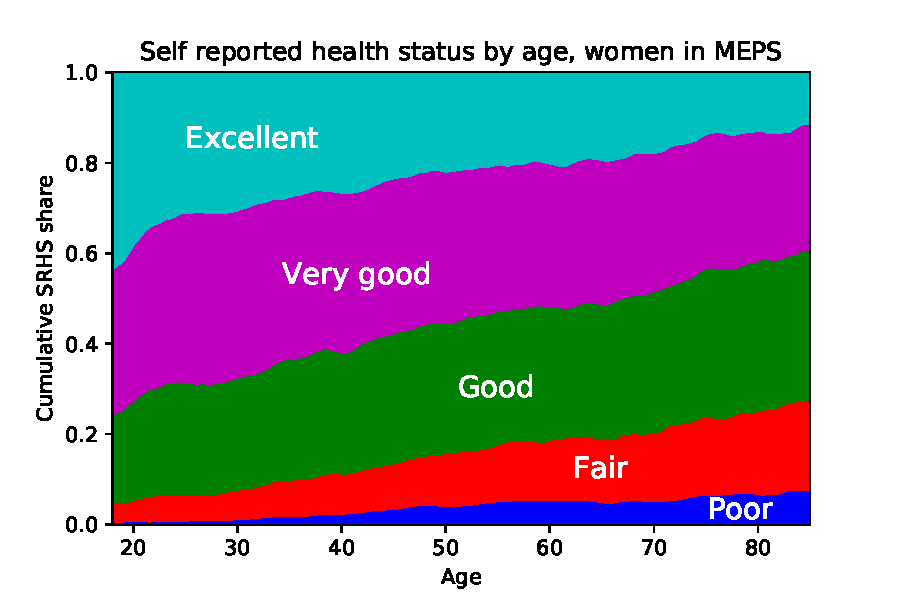
\includegraphics[scale=0.65]{\FigsDir/MEPSover18WomenSRHSbyAgeFill.pdf}
\end{center}
\end{frame}

\begin{frame}\frametitle{SRHS by age in MEPS (women)}
\begin{center}
	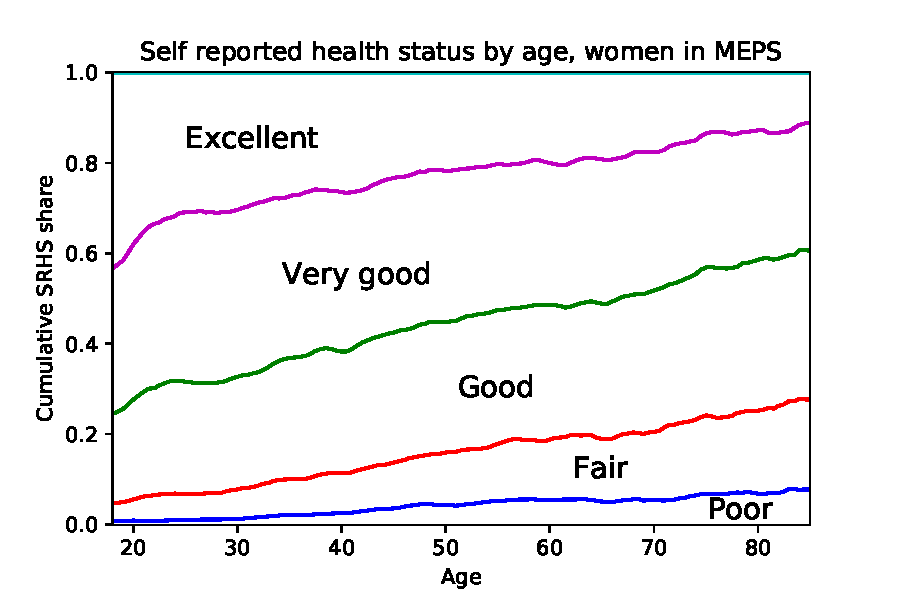
\includegraphics[scale=0.65]{\FigsDir/MEPSover18WomenSRHSbyAgeDataOnly.pdf}
\end{center}
\end{frame}


\begin{frame}\frametitle{SRHS: Actually not that bad}
\begin{itemize}
	\item <1->SRHS is \textit{highly} predictive of:
	\begin{itemize}
		\item <1->Medical expenses
		
		\item <1->Mortality
		
		\item <1->Labor supply (Bound (1991), Blundell et al (2017))
	\end{itemize}

	\item <2->\textbf{And} it's highly correlated with objective clinical measures that directly measure aspects of ``health'' (LaRue (1979))
	
	\item <3->Cheap and easy to survey, everyone understands the question, correlated with the thing we want to measure, predictive of relevant outcomes, simple to implement in models...
	
	\item <3->...So what's the problem?
\end{itemize}
\end{frame}


\subsection{Naive dynamics of SRHS}


\begin{frame}\frametitle{Standard implementation of SRHS}
\begin{itemize}
	\item <1->Most papers convert five health categories to two states:
	\begin{itemize}
		\item <1->\{Excellent, Very good, Good\} $\longrightarrow$ ``healthy''
		
		\item <1->\{Fair, Poor\} $\longrightarrow$ ``unhealthy''
	\end{itemize}
	
	\item <3->And papers take transitions between the two states ``straight from the data'':
	\begin{itemize}
		\item <3->Markov(1) process with transition probabilities calculated as a simple fraction of obs
		
		\item <3->Or maybe a reduced form model using one period transitions (smoothing probs)
	\end{itemize}
    \item <2->This is throwing out data! Losing relevant information

	\item <4->And taking SRHS \textbf{way} too literally
\end{itemize}
\end{frame}


\begin{frame}\frametitle{Taking SRHS transitions ``straight from the data''}
\begin{center}
	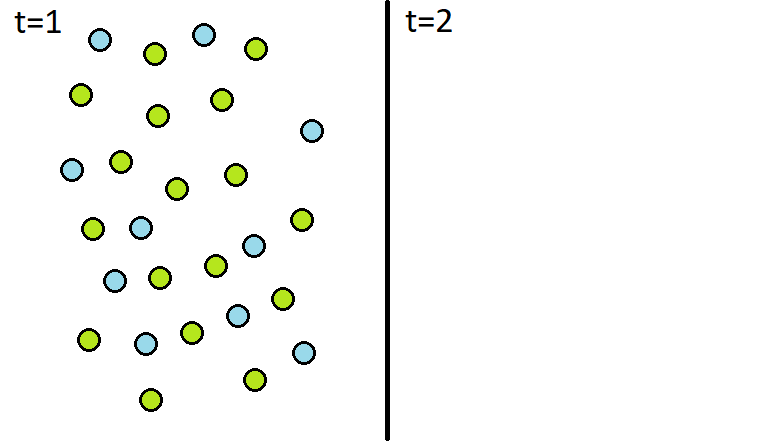
\includegraphics[scale=0.5]{\FigsDir/CountTrans0.png}
\end{center}
\end{frame}


\begin{frame}\frametitle{Taking SRHS transitions ``straight from the data''}
\begin{center}
	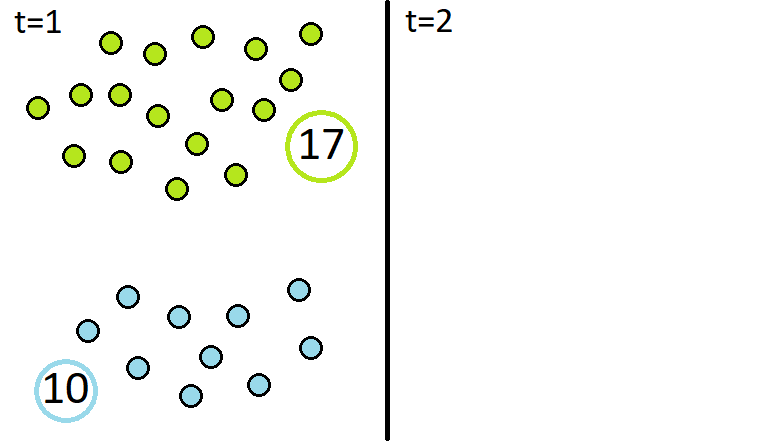
\includegraphics[scale=0.5]{\FigsDir/CountTrans1.png}
\end{center}
\end{frame}


\begin{frame}\frametitle{Taking SRHS transitions ``straight from the data''}
\begin{center}
	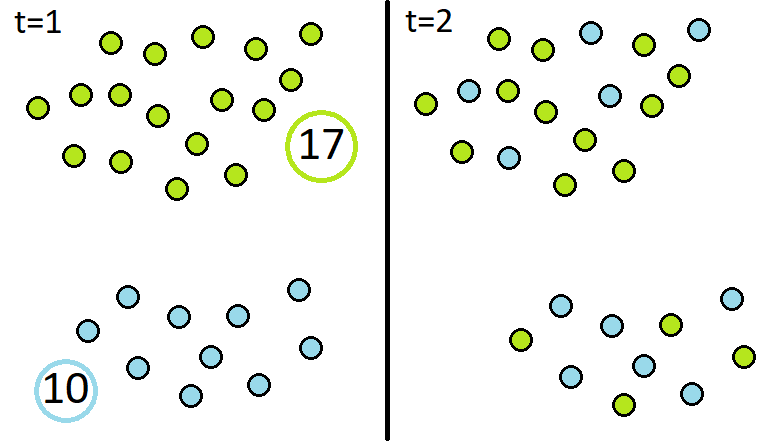
\includegraphics[scale=0.5]{\FigsDir/CountTrans2a.png}
\end{center}
\end{frame}


\begin{frame}\frametitle{Taking SRHS transitions ``straight from the data''}
\begin{center}
	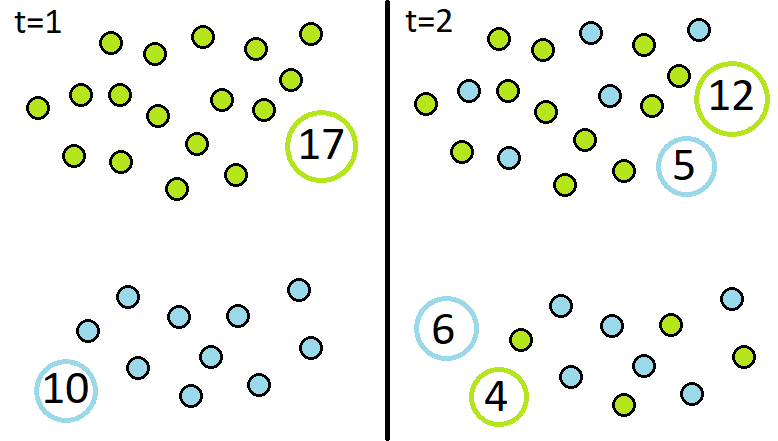
\includegraphics[scale=0.5]{\FigsDir/CountTrans2.png}
\end{center}
\end{frame}


\begin{frame}\frametitle{Taking SRHS transitions ``straight from the data''}
\begin{center}
	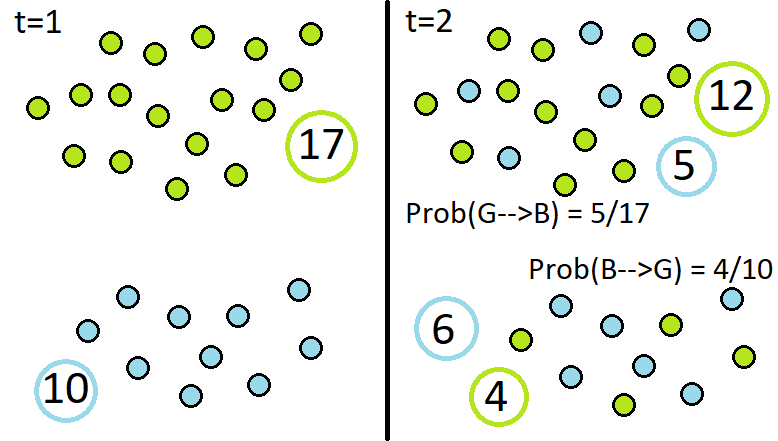
\includegraphics[scale=0.5]{\FigsDir/CountTrans3.png}
\end{center}
\end{frame}


\begin{frame}\frametitle{Taking SRHS transitions ``straight from the data''}
Probit or logit model:

\begin{equation*}
y_{t} = \beta_0 + \beta_1 age_{t-1} + \beta_2 age^2_{t-1} + \beta_3 sex + \beta_4 h_{t-1} + \epsilon_t,
\end{equation*}
\begin{equation*}
h_t = \begin{cases}
1 & \text{if } y_t < 0 \\
2 & \text{if } y_t \geq 0
\end{cases}.
\end{equation*}

Models with more than two health states use multinomial logit (e.g.\ Khwaja (2010))... but always on one period transitions
\end{frame}


\begin{frame}\frametitle{Naive SRHS transitions for MEPS women: 1 wave}
\begin{center}
	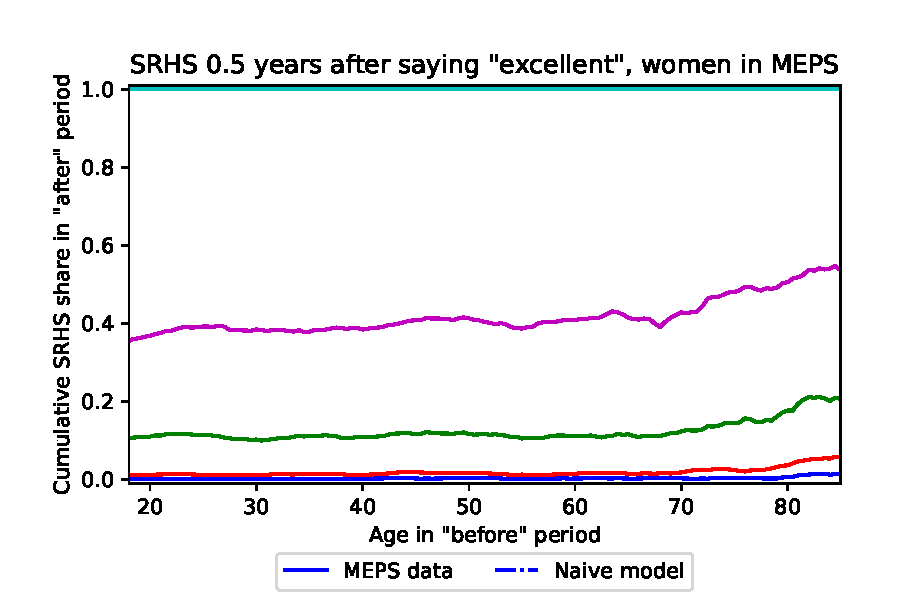
\includegraphics[scale=0.65]{\FigsDir/MEPSover18WomenTransH5T1naive.pdf}
\end{center}
\end{frame}

\begin{frame}\frametitle{Naive SRHS transitions for MEPS women: 1 wave}
\begin{center}
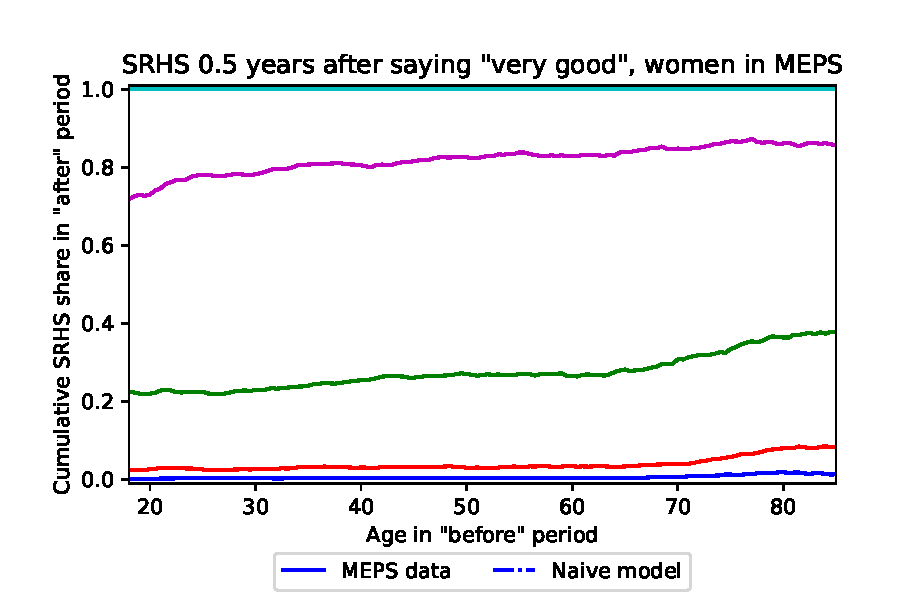
\includegraphics[scale=0.65]{\FigsDir/MEPSover18WomenTransH4T1naive.pdf}
\end{center}
\end{frame}

\begin{frame}\frametitle{Naive SRHS transitions for MEPS women: 1 wave}
\begin{center}
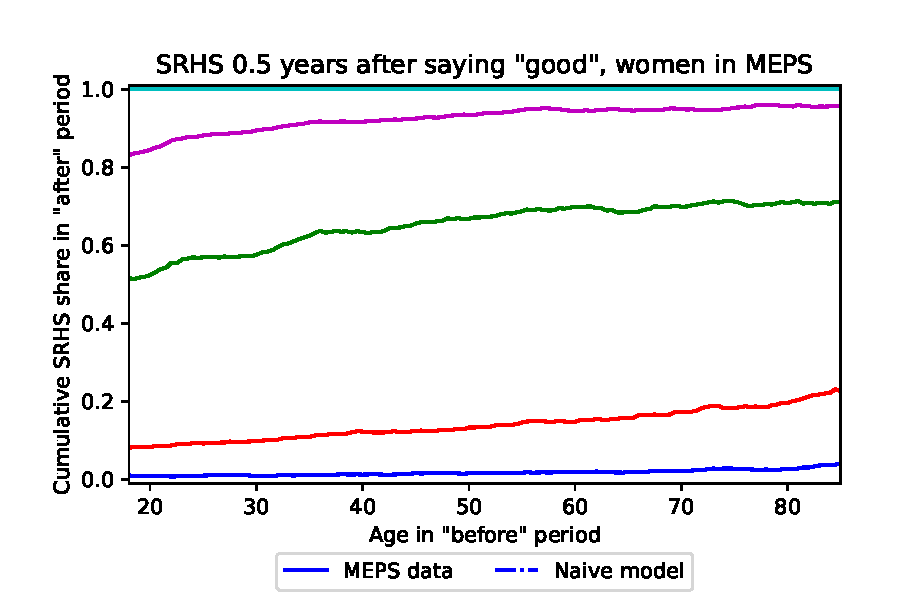
\includegraphics[scale=0.65]{\FigsDir/MEPSover18WomenTransH3T1naive.pdf}
\end{center}
\end{frame}

\begin{frame}\frametitle{Naive SRHS transitions for MEPS women: 1 wave}
\begin{center}
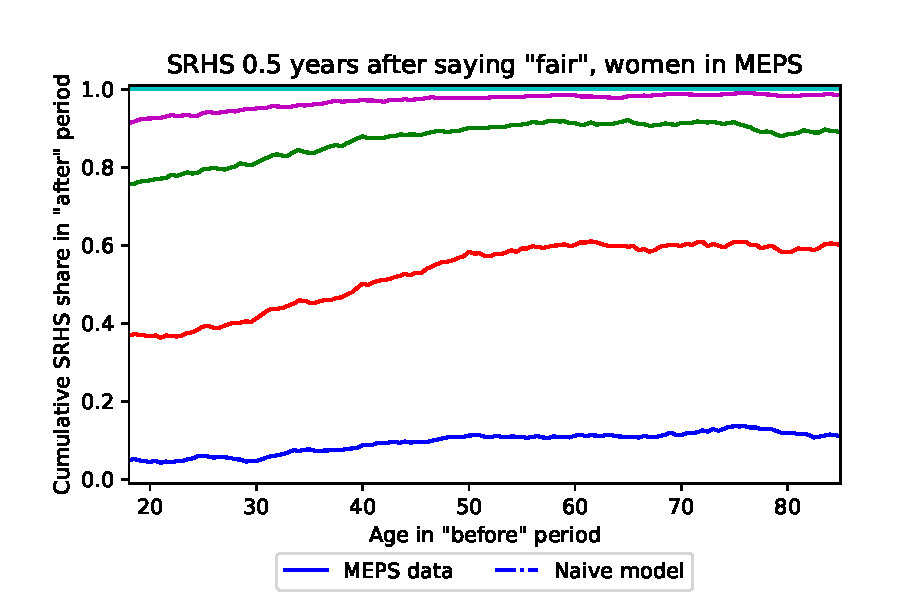
\includegraphics[scale=0.65]{\FigsDir/MEPSover18WomenTransH2T1naive.pdf}
\end{center}
\end{frame}

\begin{frame}\frametitle{Naive SRHS transitions for MEPS women: 1 wave}
\begin{center}
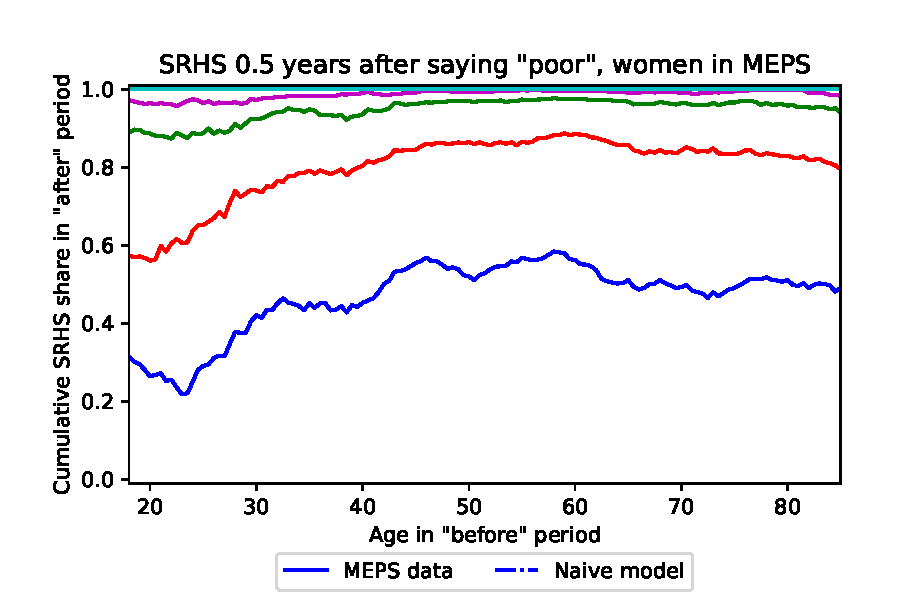
\includegraphics[scale=0.65]{\FigsDir/MEPSover18WomenTransH1T1naive.pdf}
\end{center}
\end{frame}

\begin{frame}\frametitle{Naive SRHS transitions for MEPS women: 2 waves}
\begin{center}
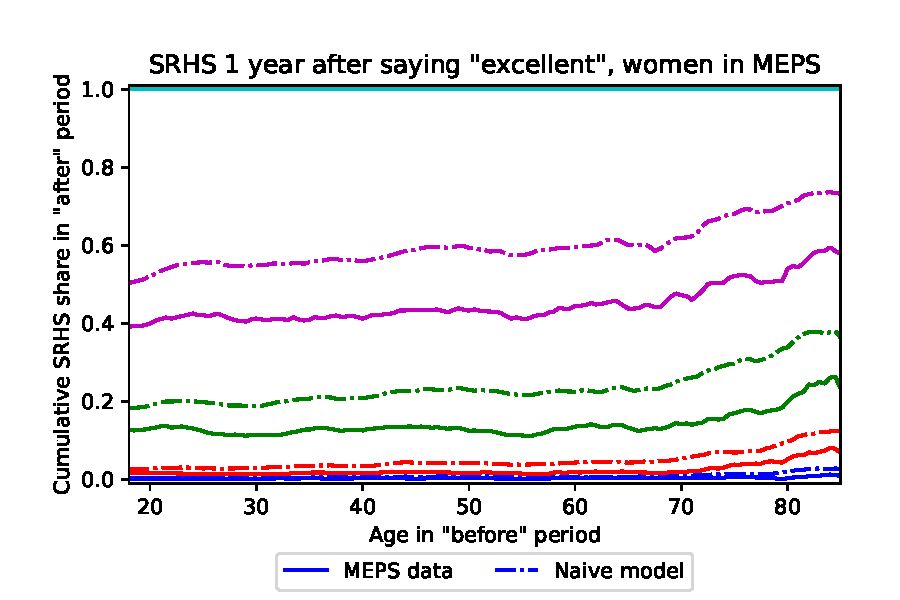
\includegraphics[scale=0.65]{\FigsDir/MEPSover18WomenTransH5T2naive.pdf}
\end{center}
\end{frame}

\begin{frame}\frametitle{Naive SRHS transitions for MEPS women: 2 waves}
\begin{center}
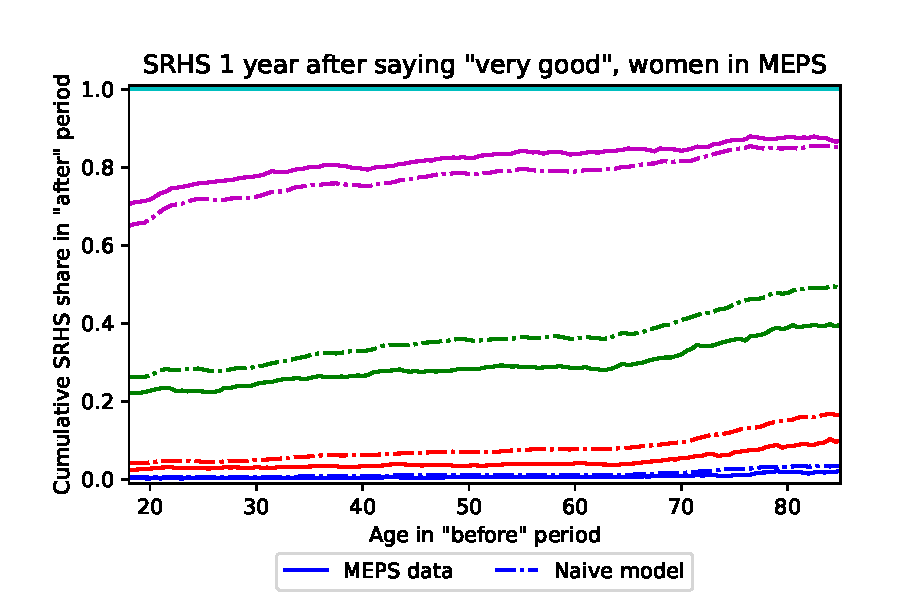
\includegraphics[scale=0.65]{\FigsDir/MEPSover18WomenTransH4T2naive.pdf}
\end{center}
\end{frame}

\begin{frame}\frametitle{Naive SRHS transitions for MEPS women: 2 waves}
\begin{center}
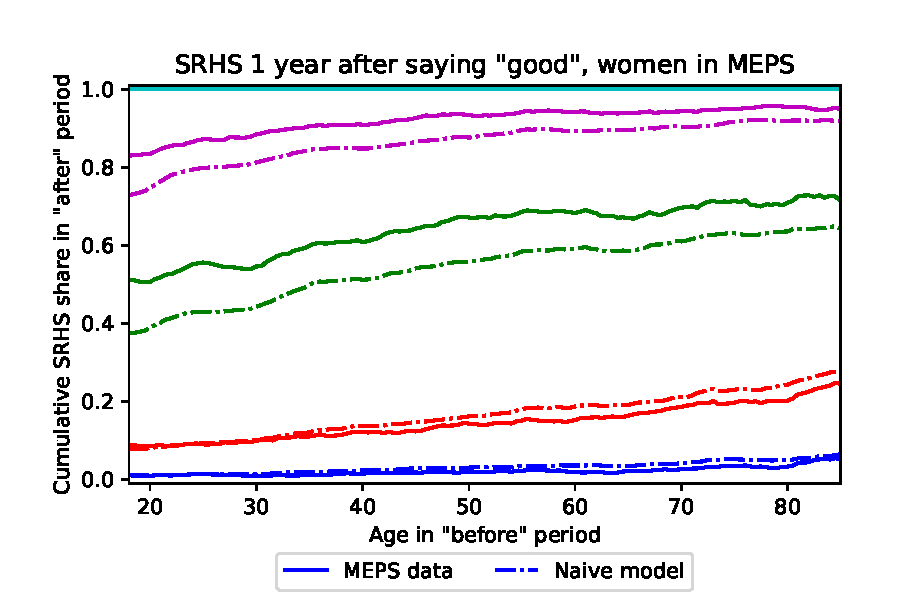
\includegraphics[scale=0.65]{\FigsDir/MEPSover18WomenTransH3T2naive.pdf}
\end{center}
\end{frame}

\begin{frame}\frametitle{Naive SRHS transitions for MEPS women: 2 waves}
\begin{center}
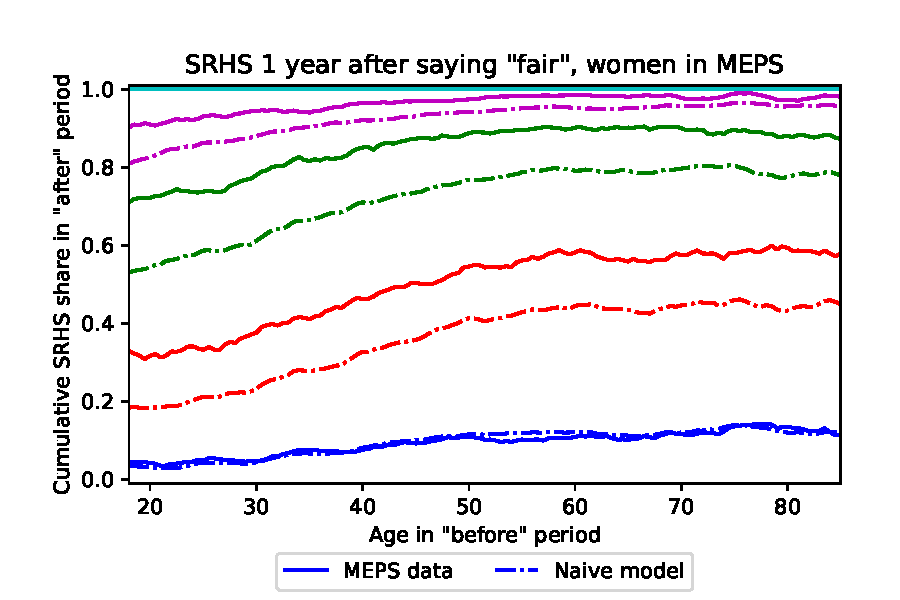
\includegraphics[scale=0.65]{\FigsDir/MEPSover18WomenTransH2T2naive.pdf}
\end{center}
\end{frame}

\begin{frame}\frametitle{Naive SRHS transitions for MEPS women: 2 waves}
\begin{center}
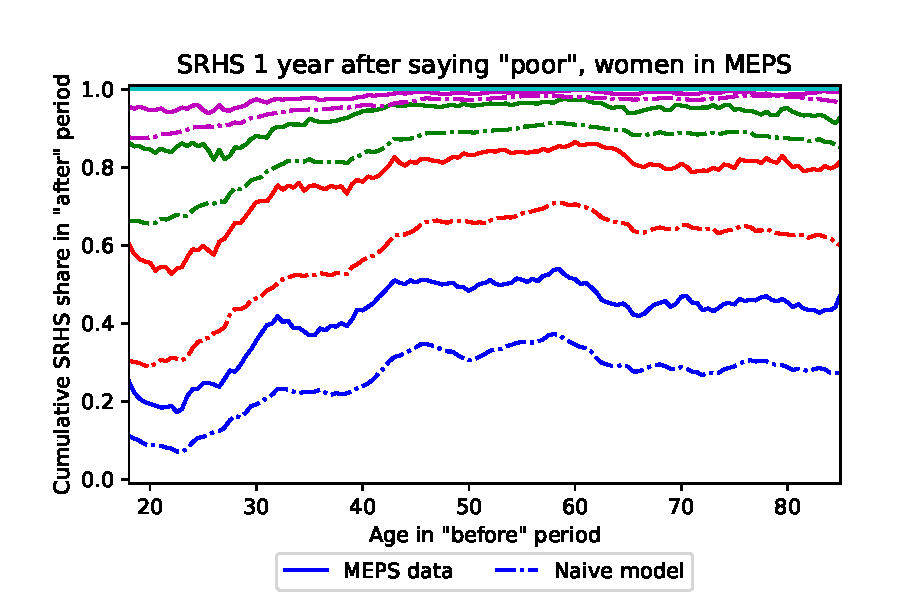
\includegraphics[scale=0.65]{\FigsDir/MEPSover18WomenTransH1T2naive.pdf}
\end{center}
\end{frame}

\begin{frame}\frametitle{Naive SRHS transitions for MEPS women: 4 waves}
\begin{center}
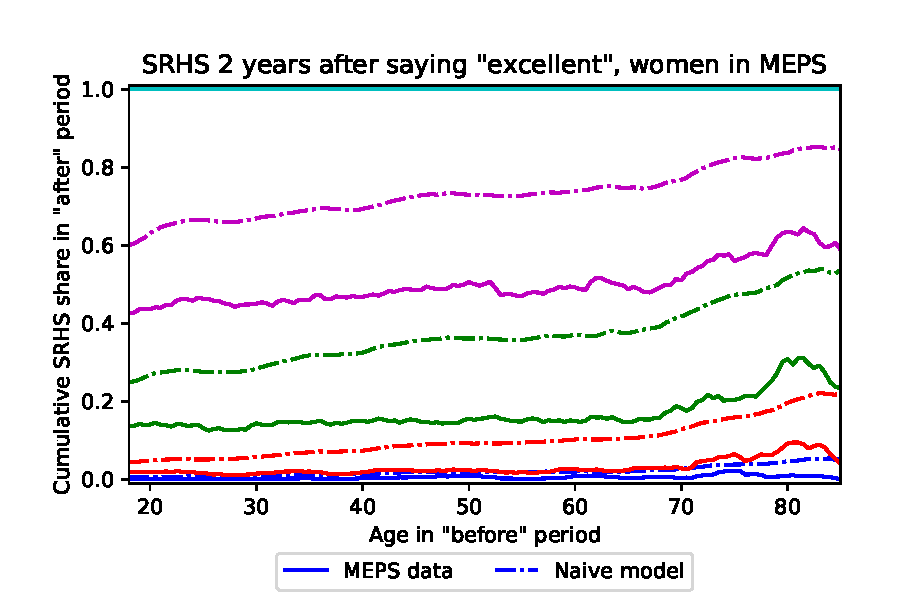
\includegraphics[scale=0.65]{\FigsDir/MEPSover18WomenTransH5T4naive.pdf}
\end{center}
\end{frame}

\begin{frame}\frametitle{Naive SRHS transitions for MEPS women: 4 waves}
\begin{center}
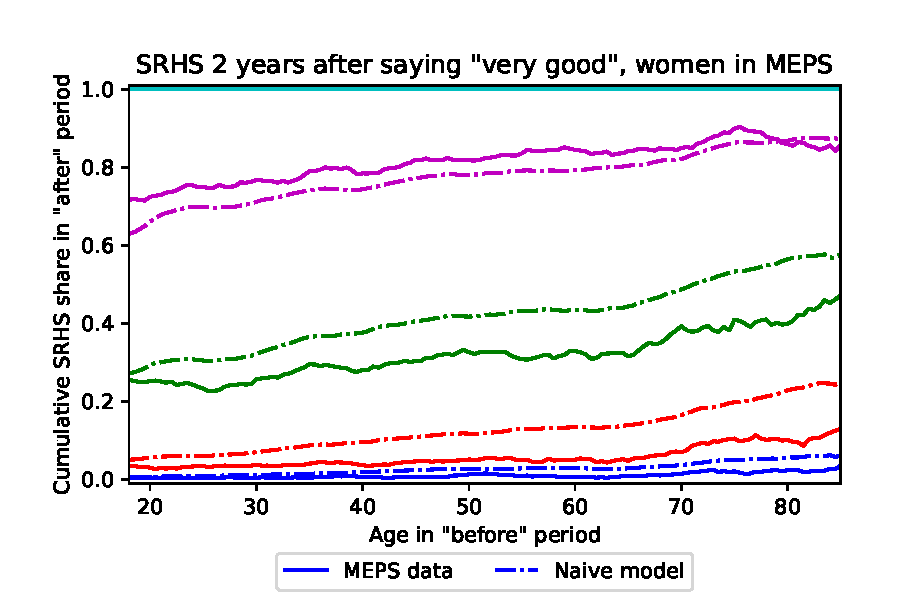
\includegraphics[scale=0.65]{\FigsDir/MEPSover18WomenTransH4T4naive.pdf}
\end{center}
\end{frame}

\begin{frame}\frametitle{Naive SRHS transitions for MEPS women: 4 waves}
\begin{center}
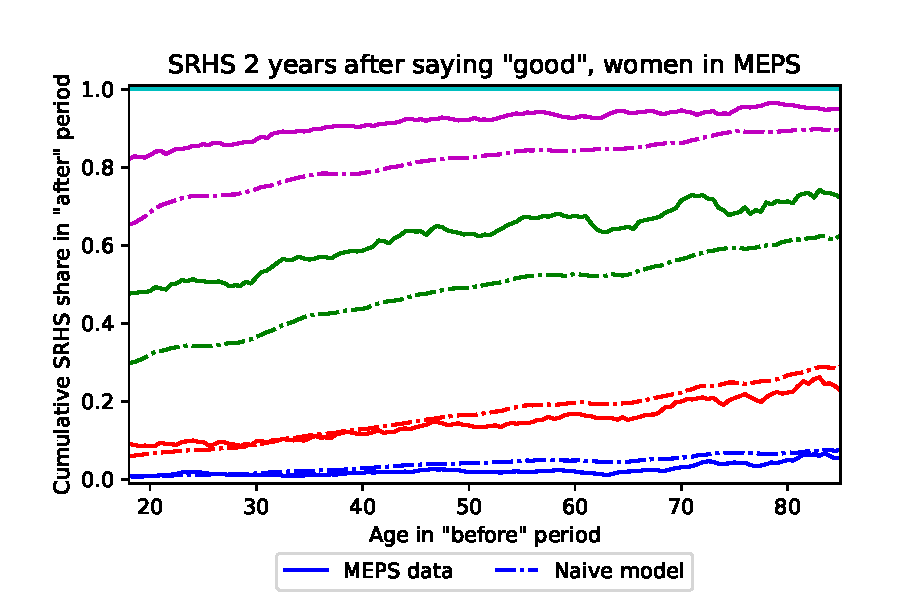
\includegraphics[scale=0.65]{\FigsDir/MEPSover18WomenTransH3T4naive.pdf}
\end{center}
\end{frame}

\begin{frame}\frametitle{Naive SRHS transitions for MEPS women: 4 waves}
\begin{center}
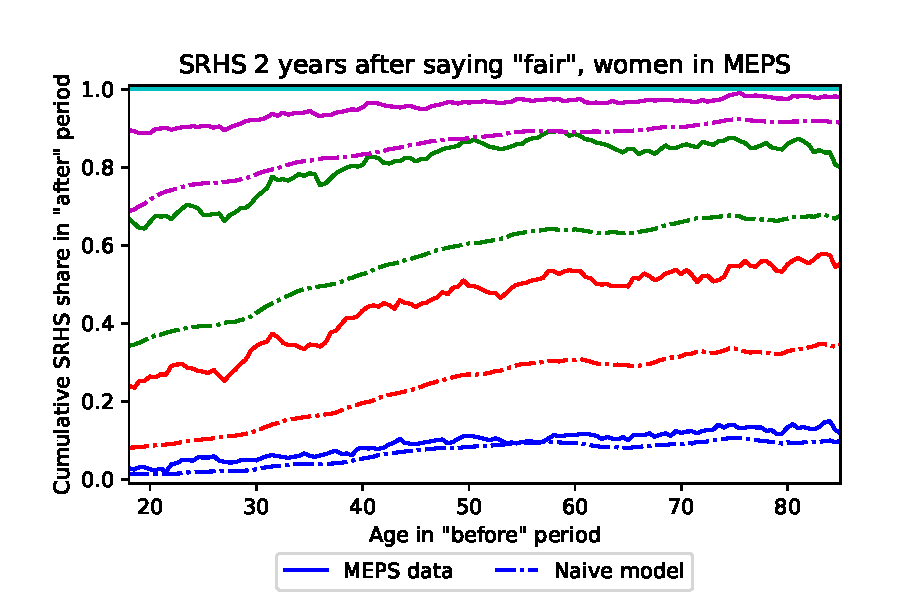
\includegraphics[scale=0.65]{\FigsDir/MEPSover18WomenTransH2T4naive.pdf}
\end{center}
\end{frame}

\begin{frame}\frametitle{Naive SRHS transitions for MEPS women: 4 waves}
\begin{center}
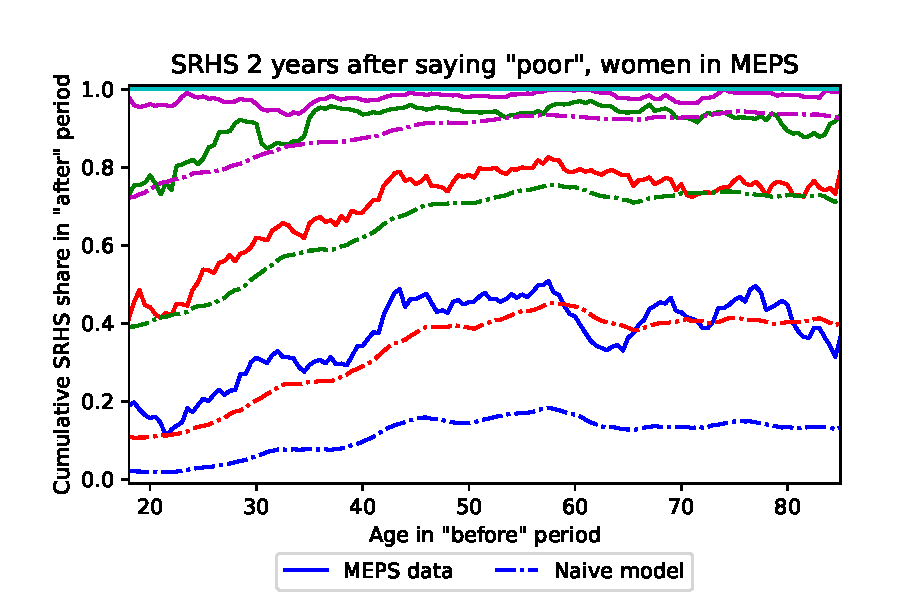
\includegraphics[scale=0.65]{\FigsDir/MEPSover18WomenTransH1T4naive.pdf}
\end{center}
\end{frame}


\begin{frame}\frametitle{Who uses naive SRHS dynamics?}

\begin{itemize}
	\item <1->Naive health transitions calculated straight from the data are \textbf{obviously} a bad idea
	
	\item <2->Who would possibly use them in ``serious'' work?
	
	\item <2->What journals would publish such papers?
\end{itemize}
\end{frame}


\begin{frame}\frametitle{Who uses naive SRHS dynamics?}

``We estimate the probability of death and bad health as logistic functions of a cubic in age, sex, sex interacted with age, previous health status, health status interacted with age, a quadratic in permanent income rank, and permanent income rank interacted with age.''
\begin{center}
	--- DeNardi, French, \& Jones (2010), J. of Political Economy
\end{center}
\end{frame}


\begin{frame}\frametitle{Who uses naive SRHS dynamics?}

	``In the first [estimation] step, we estimate or calibrate parameters that can be cleanly identified without explicitly using our model. For example, we estimate mortality rates and health transitions straight from demographic data.''
	
\begin{center}
	--- French \& Jones (2011), Econometrica
\end{center}
\end{frame}


\begin{frame}\frametitle{Who uses naive SRHS dynamics?}

``To construct the transition matrix we measure the fraction of people who move from one bin to another between two consecutive years''

\begin{center}
	--- Pashchenko \& Porapakkarm (2013), Review of Economic Dynamics
\end{center}
\end{frame}


\begin{frame}\frametitle{Who uses naive SRHS dynamics?}

``[S]ome parameters are estimated outside the structure of the model. For some parameters, this is because no structure is needed: disability risk can be estimated directly from transitions between disability states because of the exogeneity assumption.''

\begin{center}
	--- Low \& Pistaferri (2015), American Economic Review
\end{center}
\end{frame}


\begin{frame}\frametitle{Who uses naive SRHS dynamics?}

``We estimate health transitions and mortality rates simultaneously by fitting the transitions observed in the HRS to a multinomial logit model [...] on age, sex, current health status, and PI.''

\begin{center}
	--- DeNardi, French, \& Jones (2016), American Economic Review
\end{center}
\end{frame}


\begin{frame}\frametitle{Who uses naive SRHS dynamics?}

``We estimated the transition probabilities using the logit method. We regressed next period's health status on a constant, age, age squared, age cubic, education level, current health status, and age times current health status.''
\begin{center}
	--- Ferreira \& Gomes (2017), Review of Economic Dynamics
\end{center}
\end{frame}


\begin{frame}\frametitle{Who uses naive SRHS dynamics?}

``The transition to next period health status is determined as a logistic function of [math notation].''

\begin{center}
	---Aizawa (forthcoming), Quantitative Economics
\end{center}
\end{frame}



\subsection{Less naive dynamics}


\begin{frame}\frametitle{SRHS is not Markov(1) (1/3)}
\begin{itemize}
	\item <1->Markov(1) assumption means that \textbf{all} relevant information about realization of SRHS $h_t$ is contained in information at $t-1$ $(\Omega_{t-1})$
	
	\item <2->Specifically: $h_{t-n}$ for $n \geq 2$ is not predictive of $h_{t}$ if $h_{t-1}$ is known
	
	\item <3->Problem: That's just not true
\end{itemize}
\end{frame}


\begin{frame}\frametitle{SRHS is not Markov(1) (2/3)}
\begin{itemize}
	\item <1->MEPS: Respondents interviewed five times over two years (6 month waves); new Panel started each year from 1996 onward
	
	\item <1->Example: Women between ages 40-45 in Panels 1-20
	
	\item <2->Probability of reporting SRHS ``unhealthy'' at wave 5 conditional on reporting ``unhealthy'' at wave 4: 74.7\%
	
	\item <3->...\textbf{and} reporting ``unhealthy'' at wave 3: 80.1\%
	
	\item <4->...\textbf{and} reporting ``unhealthy'' at wave 2: 81.8\%
	
	\item <5->...\textbf{and} reporting ``unhealthy'' at wave 1: 84.6\%
\end{itemize}
\end{frame}


\begin{frame}\frametitle{SRHS is not Markov(1) (3/3)}
DeNardi, Pashchenko, and Porapakkarm (2018): This is evidence of \textit{duration dependence} in health, so let's make transition probabilities dependent on duration (plus add heterogeneity)!
\begin{center}
	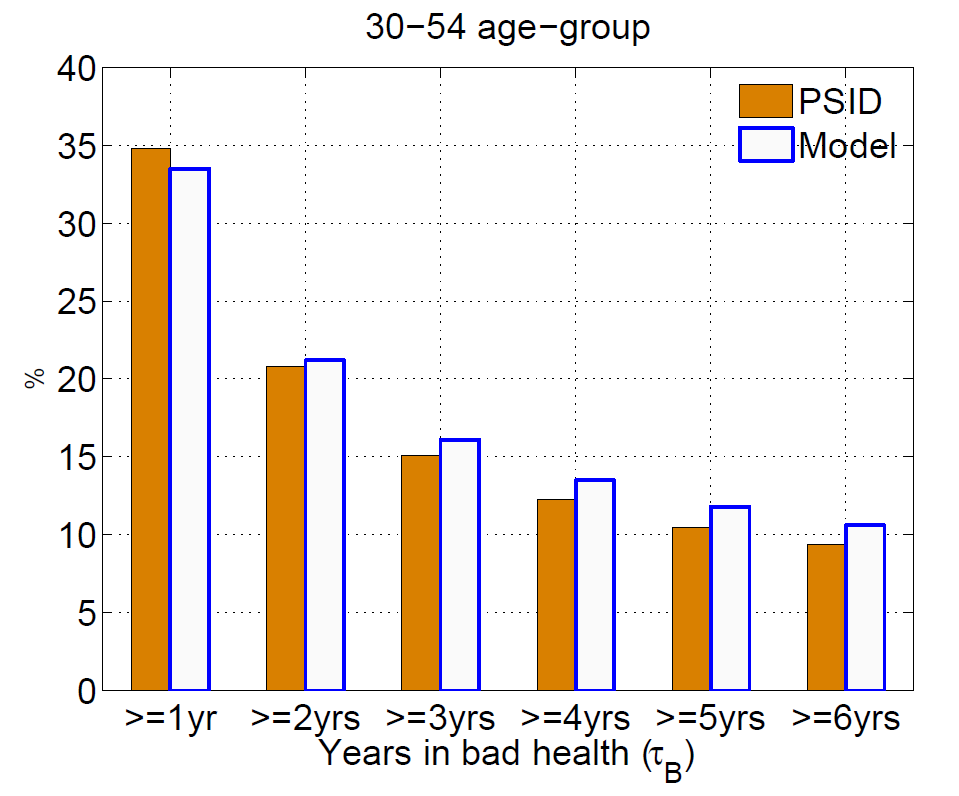
\includegraphics[scale=0.25]{\FigsDir/PPandDeNardiA.png}
\end{center}
\end{frame}


\begin{frame}\frametitle{SRHS is not Markov(1) (3/3)}
DeNardi, Pashchenko, and Porapakkarm (2018): This is evidence of \textit{duration dependence} in health, so let's make transition probabilities dependent on duration (plus add heterogeneity)!
\begin{center}
	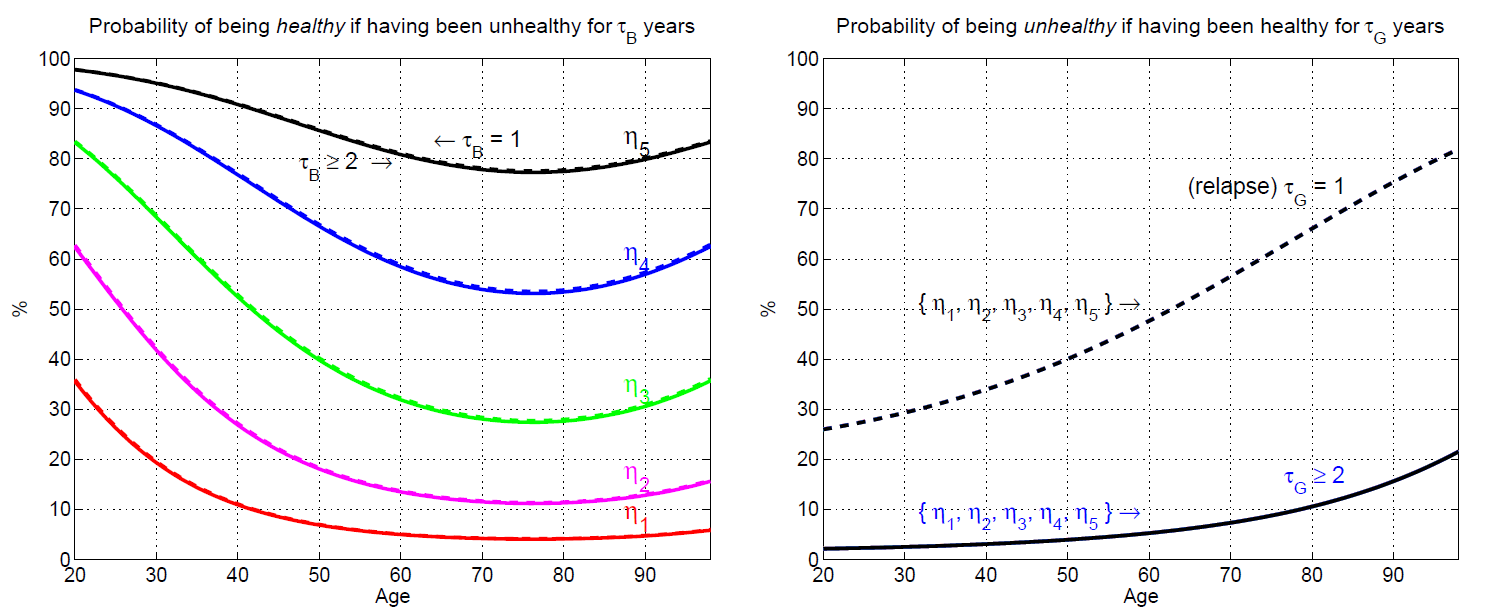
\includegraphics[scale=0.30]{\FigsDir/PPandDeNardiB.png}
\end{center}
\end{frame}


\begin{frame}\frametitle{But it's not duration dependence (1/3)}
\begin{itemize}
	\item <1->DeNardi et al model health transitions between two states as Markov(2): $h_{t}$ probabilities depend on $h_{t-1}$ and $h_{t-2}$...
	
	\item <2->...But still treat ``healthy'' and ``unhealthy'' as the only states: mortality and medical expense distribution depend on $h_t$ only!
	
	\item <3->This is easily falsifiable; quick example with early 40's women:
	
	\item <3->Mean log medical costs for ``unhealthy'': 7.80
	\begin{itemize}
		\item <4->...and ``unhealthy'' one year prior: 7.95
		
		\item <4->...and ``healthy'' one year prior: 7.57
	\end{itemize}

	\item <3->Mean log medical costs for ``healthy'': 6.82
	\begin{itemize}
		\item <5->...and ``unhealthy'' one year prior: 7.14
		
		\item <5->...and ``healthy'' one year prior: 6.79
	\end{itemize}
	
	\item <6->\textbf{Lagged SRHS generates observably different medical expense distributions; ``unhealthy'' people are not all in the same health state!}
\end{itemize}
\end{frame}


\begin{frame}\frametitle{But it's not duration dependence  (2/3)}
\begin{itemize}
	\item <1->Let's take another look at those early 40's MEPS women
	
	\item <1->Probability of reporting SRHS ``unhealthy'' at wave 1 conditional on reporting ``unhealthy'' at wave 1: 100.0\%
	
	\item <2->Probability of reporting SRHS ``unhealthy'' at wave 2 conditional on reporting ``unhealthy'' at wave 1: 57.9\%
	
	\item <3->Probability of reporting SRHS ``unhealthy'' at wave 3 conditional on reporting ``unhealthy'' at wave 1: 57.6\%
	
	\item <4->Probability of reporting SRHS ``unhealthy'' at wave 4 conditional on reporting ``unhealthy'' at wave 1: 56.7\%
	
	\item <5->Probability of reporting SRHS ``unhealthy'' at wave 5 conditional on reporting ``unhealthy'' at wave 1: 55.8\%
	
	\item <6->\textbf{Wave 1 SRHS is nearly as predictive of W5 SRHS as it is for W2 SRHS!}
\end{itemize}
\end{frame}


\begin{frame}\frametitle{But it's not duration dependence (3/3)}
\begin{itemize}
	\item <1->Suppose you saw these examples, but the labels were ``in bottom income quintile'' and ``above bottom income quintile''
	
	\item <2->You would not hypothesize: ``There must be duration dependence in being poor!''
	
	\item <3->Income quintile is a discretization of continuous income
	
	\item <3->SRHS is a discretization of continuous ``health''
	
	\item <4->Income changes with both permanent and transitory shocks
	
	\item <4->SRHS changes with both changes in ``true health'' and transitory \textbf{reporting} shocks
\end{itemize}
\end{frame}


\section{Model \& Likelihood}


\begin{frame}
\begin{center}
\Huge
MODEL
\end{center}
\end{frame}

\subsection{Graphical model}


\begin{frame}\frametitle{Graphical model of latent health and SRHS (1/5)}
``True health'' lives in some weird polydimensional space \\ \hspace{0.5cm}
\begin{center}
	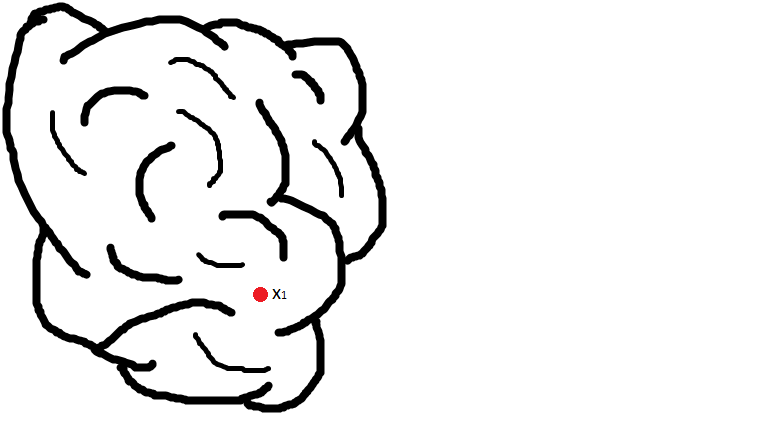
\includegraphics[scale=0.5]{\FigsDir/TrueHealth1.png}
\end{center}
\end{frame}


\begin{frame}\frametitle{Graphical model of latent health and SRHS (2/5)}
Dynamics of ``true health'' really \textbf{are} Markov(1) \\ \hspace{0.5cm}
\begin{center}
	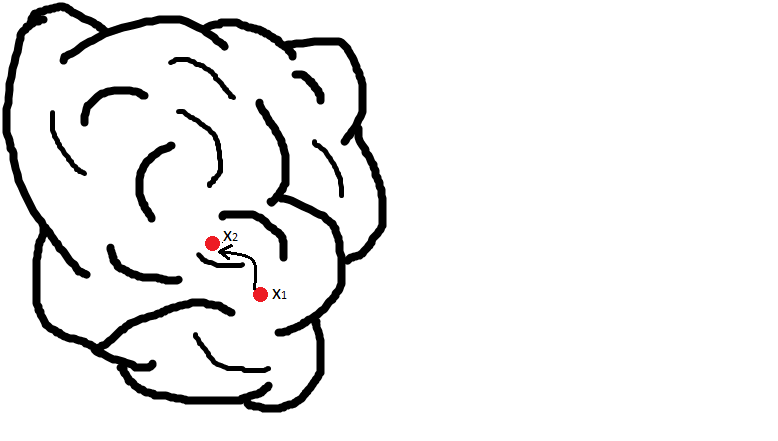
\includegraphics[scale=0.5]{\FigsDir/TrueHealth2.png}
\end{center}
\end{frame}

\begin{frame}\frametitle{Graphical model of latent health and SRHS (2/5)}
Dynamics of ``true health'' really \textbf{are} Markov(1) \\ \hspace{0.5cm}
\begin{center}
	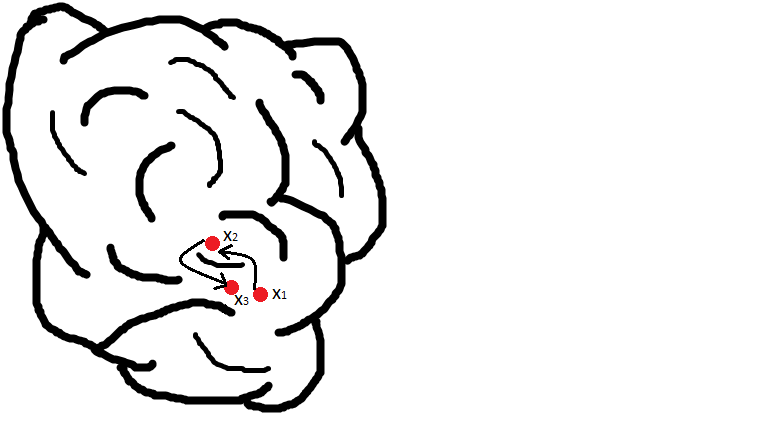
\includegraphics[scale=0.5]{\FigsDir/TrueHealth3.png}
\end{center}
\end{frame}

\begin{frame}\frametitle{Graphical model of latent health and SRHS (2/5)}
Dynamics of ``true health'' really \textbf{are} Markov(1) \\ \hspace{0.5cm}
\begin{center}
	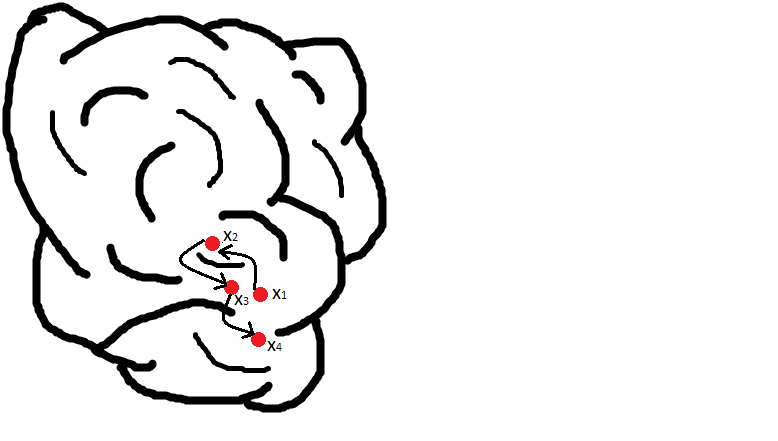
\includegraphics[scale=0.5]{\FigsDir/TrueHealth4.png}
\end{center}
\end{frame}


\begin{frame}\frametitle{Graphical model of latent health and SRHS (3/5)}
SRHS is a projection of that polydimensional space \\ onto a discrete space...
\begin{center}
	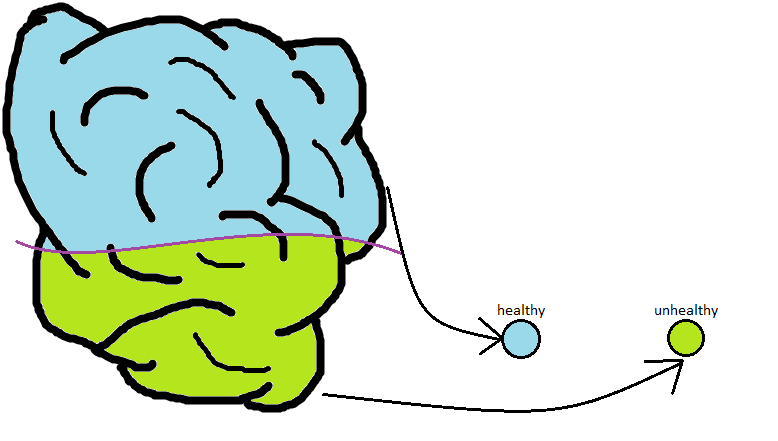
\includegraphics[scale=0.5]{\FigsDir/TrueHealthSplit.png}
\end{center}
\end{frame}

\begin{frame}\frametitle{Graphical model of latent health and SRHS (3/5)}
SRHS is a projection of that polydimensional space \\ onto a discrete space... with reporting error
\begin{center}
	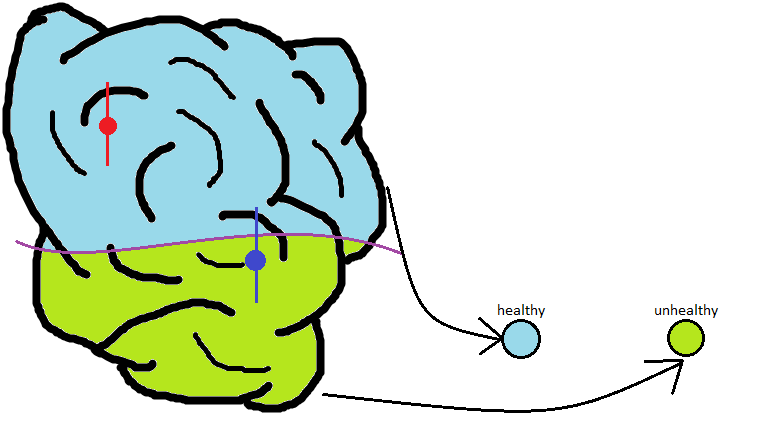
\includegraphics[scale=0.5]{\FigsDir/TrueHealthReport.png}
\end{center}
\end{frame}


\begin{frame}\frametitle{Graphical model of latent health and SRHS (4/5)}
Individuals whose ``true health'' is far from the healthy/unhealthy threshold are likely to have the same SRHS period after period
\begin{center}
	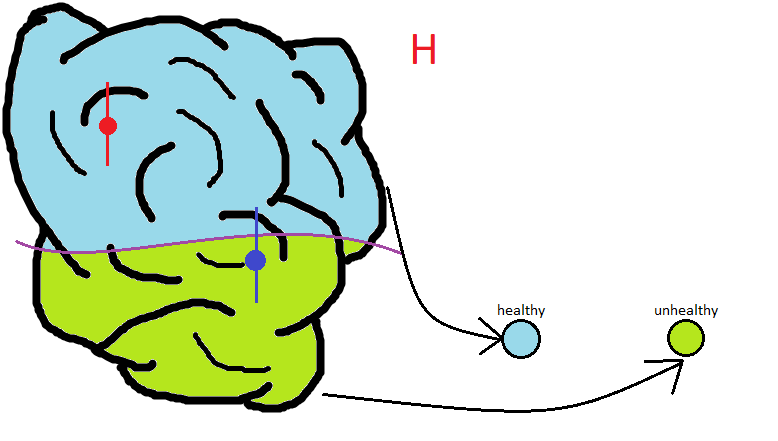
\includegraphics[scale=0.5]{\FigsDir/TrueHealthHist1.png}
\end{center}
\end{frame}

\begin{frame}\frametitle{Graphical model of latent health and SRHS (4/5)}
Individuals whose ``true health'' is far from the healthy/unhealthy threshold are likely to have the same SRHS period after period
\begin{center}
	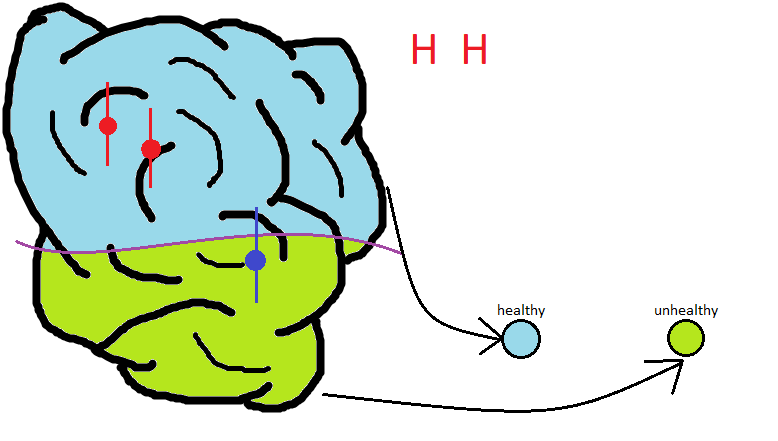
\includegraphics[scale=0.5]{\FigsDir/TrueHealthHist2.png}
\end{center}
\end{frame}

\begin{frame}\frametitle{Graphical model of latent health and SRHS (4/5)}
Individuals whose ``true health'' is far from the healthy/unhealthy threshold are likely to have the same SRHS period after period
\begin{center}
	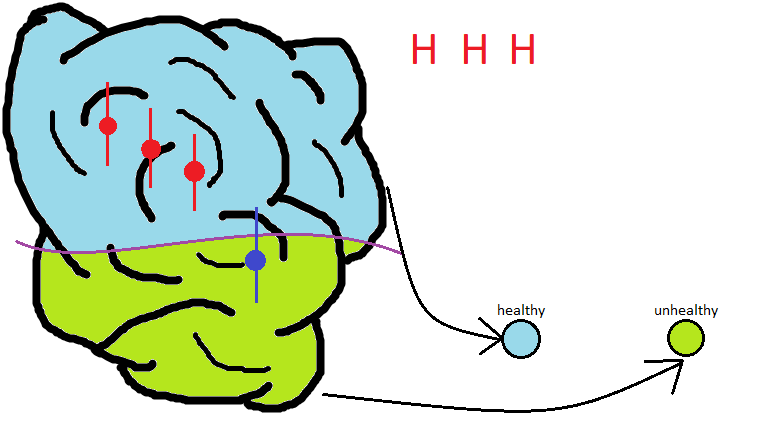
\includegraphics[scale=0.5]{\FigsDir/TrueHealthHist3.png}
\end{center}
\end{frame}

\begin{frame}\frametitle{Graphical model of latent health and SRHS (4/5)}
Individuals whose ``true health'' is far from the healthy/unhealthy threshold are likely to have the same SRHS period after period
\begin{center}
	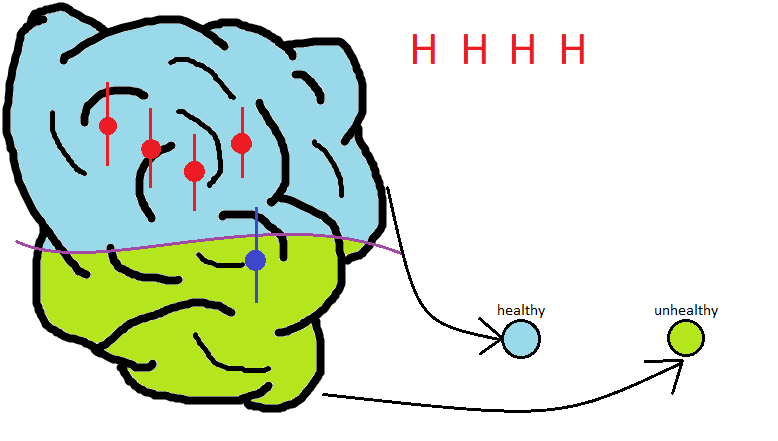
\includegraphics[scale=0.5]{\FigsDir/TrueHealthHist4.png}
\end{center}
\end{frame}

\begin{frame}\frametitle{Graphical model of latent health and SRHS (4/5)}
Individuals whose ``true health'' is far from the healthy/unhealthy threshold are likely to have the same SRHS period after period
\begin{center}
	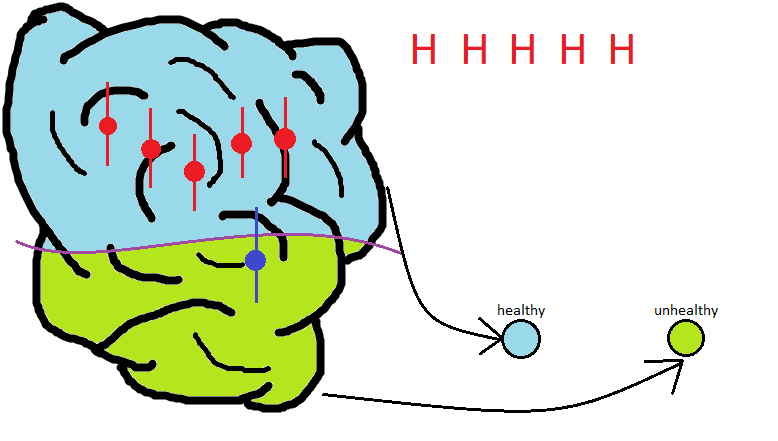
\includegraphics[scale=0.5]{\FigsDir/TrueHealthHist5.png}
\end{center}
\end{frame}

\begin{frame}\frametitle{Graphical model of latent health and SRHS (4/5)}
Individuals whose ``true health'' is far from the healthy/unhealthy threshold are likely to have the same SRHS period after period
\begin{center}
	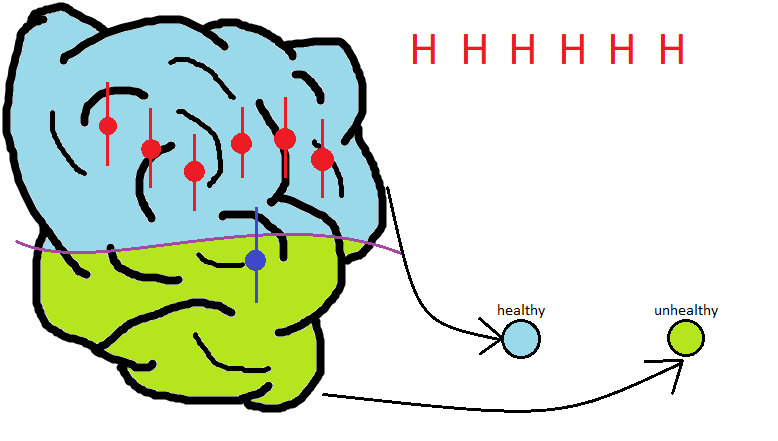
\includegraphics[scale=0.5]{\FigsDir/TrueHealthHist6.png}
\end{center}
\end{frame}


\begin{frame}\frametitle{Graphical model of latent health and SRHS (5/5)}
Individuals whose ``true health'' is close to the healthy/unhealthy threshold are more likely to change their SRHS back and forth
\begin{center}
	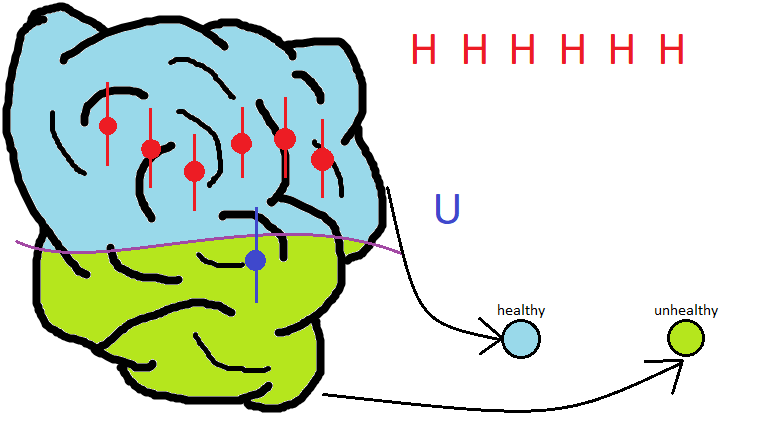
\includegraphics[scale=0.5]{\FigsDir/TrueHealthHist7.png}
\end{center}
\end{frame}

\begin{frame}\frametitle{Graphical model of latent health and SRHS (5/5)}
Individuals whose ``true health'' is close to the healthy/unhealthy threshold are more likely to change their SRHS back and forth
\begin{center}
	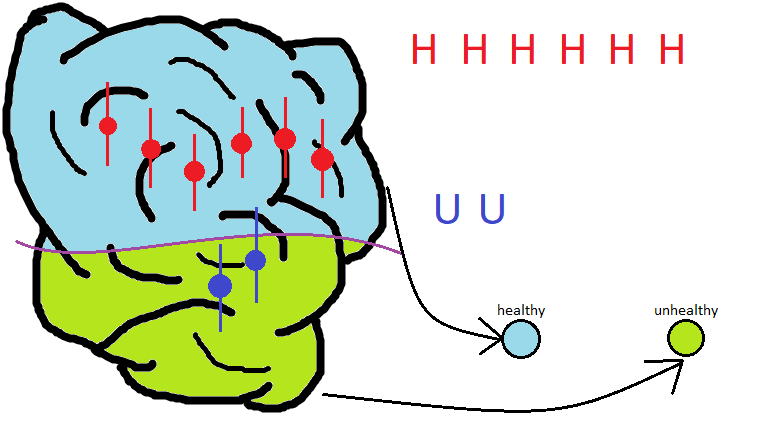
\includegraphics[scale=0.5]{\FigsDir/TrueHealthHist8.png}
\end{center}
\end{frame}

\begin{frame}\frametitle{Graphical model of latent health and SRHS (5/5)}
Individuals whose ``true health'' is close to the healthy/unhealthy threshold are more likely to change their SRHS back and forth
\begin{center}
	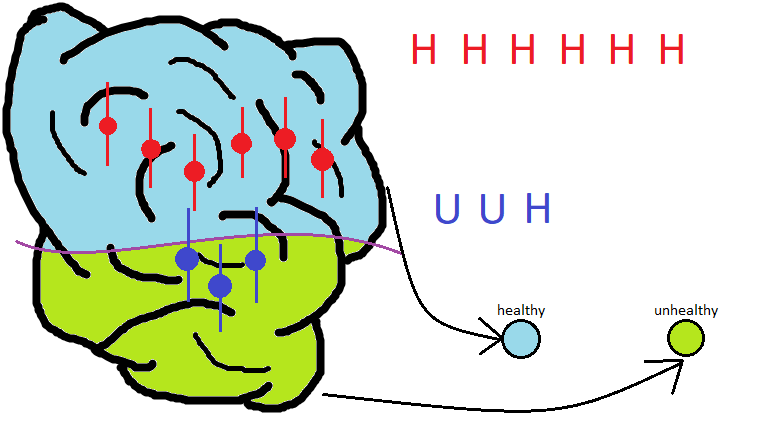
\includegraphics[scale=0.5]{\FigsDir/TrueHealthHist9.png}
\end{center}
\end{frame}

\begin{frame}\frametitle{Graphical model of latent health and SRHS (5/5)}
Individuals whose ``true health'' is close to the healthy/unhealthy threshold are more likely to change their SRHS back and forth
\begin{center}
	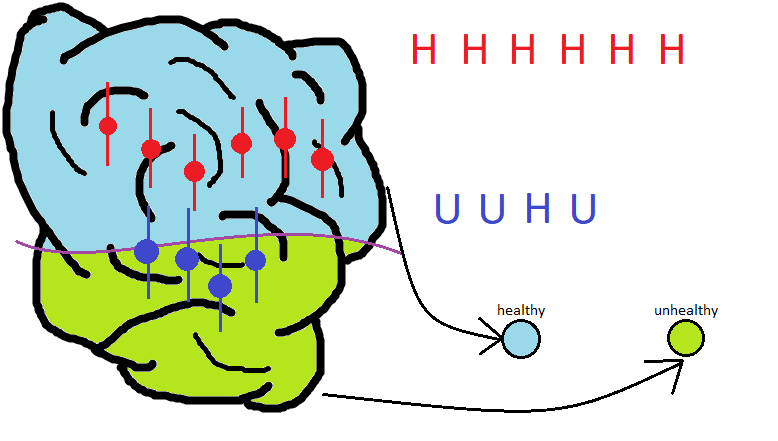
\includegraphics[scale=0.5]{\FigsDir/TrueHealthHist10.png}
\end{center}
\end{frame}

\begin{frame}\frametitle{Graphical model of latent health and SRHS (5/5)}
Individuals whose ``true health'' is close to the healthy/unhealthy threshold are more likely to change their SRHS back and forth
\begin{center}
	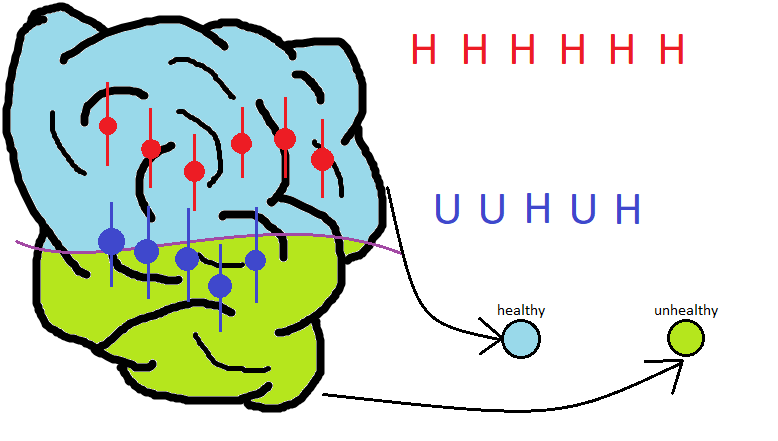
\includegraphics[scale=0.5]{\FigsDir/TrueHealthHist11.png}
\end{center}
\end{frame}

\begin{frame}\frametitle{Graphical model of latent health and SRHS (5/5)}
Individuals whose ``true health'' is close to the healthy/unhealthy threshold are more likely to change their SRHS back and forth
\begin{center}
	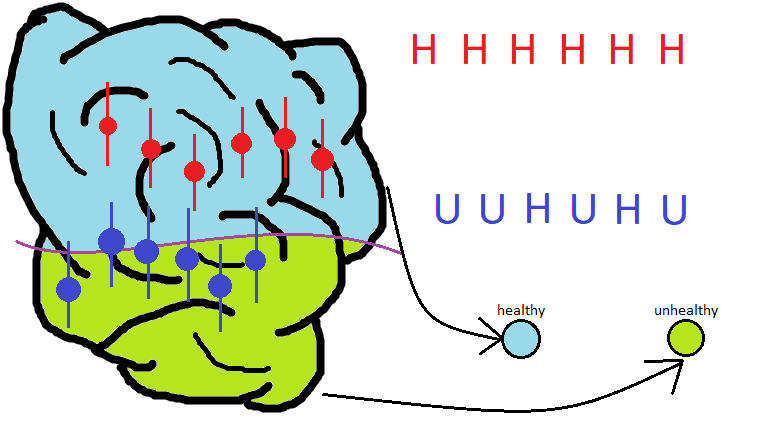
\includegraphics[scale=0.5]{\FigsDir/TrueHealthHist12.png}
\end{center}
\end{frame}


\subsection{Mathematical model}


\begin{frame}\frametitle{Feasible modeling}
\begin{itemize}
	\item <1->Polydimensional space would be hard to model
	
	\item <1->No way to estimate that model with only SRHS anyway
	
	\item <2->Feasible: one factor latent health model
	
	\item <3->Will estimate by maximum likelihood: probability of observing \textbf{sequences} of SRHS in panel data
	
	\item <3->Track (nonparametric) posterior distribution of latent health across waves for each respondent
	
	\item <4->No (unobserved) heterogeneous types
\end{itemize}
\end{frame}


\begin{frame}\frametitle{Mathematical model of latent health and SRHS}
One factor latent health model:
\begin{enumerate}
	\item <1->Distribution of latent health at model start $x_0$ is normal
	
	\item <2->Survival to next period is a probit on age $j_t$ and $x_t$
	
	\item <3->Latent health dynamics are AR(1) with standard normal shock
	
	\item <4->SRHS is an ordered probit on a linear function of $x_t$ with standard normal error
\end{enumerate}
\end{frame}


\begin{frame}\frametitle{Mathematical model of latent health and SRHS}
One factor latent health model:
\begin{equation}
x_0 \sim N(\mu_0, \sigma^2_0).
\end{equation}

\begin{enumerate}
	\setcounter{enumi}{1}
	\item Survival to next period is a probit on age $j_t$ and $x_t$
	
	\item Latent health dynamics: AR(1) with standard normal shock
	
	\item SRHS is an ordered probit on linear function of $x_t$ with standard normal error
\end{enumerate}
\end{frame}


\begin{frame}\frametitle{Mathematical model of latent health and SRHS}
One factor latent health model:
\setcounter{equation}{0}
\begin{equation}
x_0 \sim N(\mu_0, \sigma^2_0).
\end{equation}

\begin{equation}
\Prob(h_{t+1} = 0) = 1 - \Phi(f(j_t,x_t)).
\end{equation}

\begin{enumerate}
	\setcounter{enumi}{2}
	\item Latent health dynamics: AR(1) with standard normal shock
	
	\item SRHS is an ordered probit on linear function of $x_t$ with standard normal error
\end{enumerate}
\end{frame}


\begin{frame}\frametitle{Mathematical model of latent health and SRHS}
One factor latent health model:
\setcounter{equation}{0}
\begin{equation}
x_0 \sim N(\mu_0, \sigma^2_0).
\end{equation}

\begin{equation}
\Prob(h_{t+1} = 0) = 1 - \Phi(f(j_t,x_t)).
\end{equation}

\begin{equation}
x_{t+1} = \rho_{j} x_t + (1-\rho_j)g(j_t) + \epsilon_{t+1}, \qquad \epsilon_{t+1} \sim \Phi.
\end{equation}

\begin{enumerate}
	\setcounter{enumi}{3}
	\item SRHS is an ordered probit on linear function of $x_t$ with standard normal error
\end{enumerate}
\end{frame}


\begin{frame}\frametitle{Mathematical model of latent health and SRHS}
One factor latent health model:
\setcounter{equation}{0}
\begin{equation}
x_0 \sim N(\mu_0, \sigma^2_0).
\end{equation}

\begin{equation}
\Prob(h_{t+1} = 0) = 1 - \Phi(f(j_t,x_t)).
\end{equation}

\begin{equation}
x_{t+1} = \rho_{j} x_t + (1-\rho_j)g(j_t) + \epsilon_{t+1}, \qquad \epsilon_{t+1} \sim \Phi.
\end{equation}

\begin{equation}
h^*_t = \alpha_0 + \alpha_1 x_t + \eta_t, \qquad \eta_t \sim \Phi,
\end{equation}
\begin{equation*}
h_t = 1 + \sum_{k = 1}^{K-1} \mathbf{1}(h^*_t \geq \chi_k). 
\end{equation*}
\end{frame}


\begin{frame}\frametitle{Why reporting error?}
\begin{itemize}
	\item <1->Why model SRHS with reporting error?  Or: Why is it not transitory shocks to true health?
	
	\item <2->Crossley \& Kennedy (2002): 28\% of respondents \textbf{change their SRHS} if asked again later in the same interview
	
	\item <3->MEPS mails short self-administered questionnaire (SAQ) to all respondents shortly after waves 2 and 4; about 75\% response rate
	
	\item <3->Includes \textbf{nearly} identical SRHS question as main MEPS
	
	\item <4->Early 40's women: 37-38\% change SRHS from their answer a couple weeks prior if reported poor to very good health; 44\% change answer if reported excellent health
\end{itemize}
\end{frame}


\begin{frame}\frametitle{Identifying assumptions and functional forms}
\begin{itemize}
	\item <1->Mortality probit $f(\cdot)$ is polynomial of age and latent health plus linear interaction term (parameterized by $\theta$).
	
	\item <2->Latent health correlation coefficient $\rho_j$ is polynomial of age (parameterized by $\gamma$).
	
	\item <3->Latent health regression term $g(j_t)$ is polynomial of age (parameterized by $\beta$).
	
	\item <4->Scale of $x_t$ already pinned down because $\epsilon_{t+1} \sim \Phi$.
	
	\item <4->Fix location of $x_t$ by setting $\alpha_0 = 0$ and $\chi_1 = 0$.
	
	\item <5->All parameters can differ between men and women.
	
	\item <5->No reporting error for mortality.
	
	\item <5->No selection in attrition or missing SRHS.
\end{itemize}
\end{frame}



\subsection{Likelihood function}


\begin{frame}\frametitle{Log likelihood function: Precomputation}
\begin{itemize}
	\item <1->Can estimate latent health model using maximum likelihood
	
	\item <2->Slice space of latent health $x_t$ into many bins (150)
	
	\item <2->Choose some very old age that no one in data reaches
	
	\item <3->Given a vector of parameter guess $(\theta, \gamma, \beta, \alpha, \chi, \mu_0,\sigma_0)$, can precompute arrays:
	\begin{enumerate}
		\item <3->Initial pmf of $x_t$ at model start (age ``0'')
		
		\item <4->Survival probability for every $x_t$ and age $j_t$
		
		\item <4->Transition probability from every $x_t$ to every $x_{t+1}$ at every age
		
		\item <5->Probability of reporting each SRHS $h_t$ conditional on $x_t$
	\end{enumerate}

	\item <6->Using (1-3), can precompute \textbf{unconditional} pmf of $x_t$ at every age (i.e.\ simulation by multiplication)
\end{itemize}
\end{frame}


\begin{frame}\frametitle{Log likelihood function: Observation likelihood}
For each individual in the data:
\begin{enumerate}
	\item <1->Initialize ``survival probability since last observation'' to 1.0
	
	\item <1->Get precomputed pmf of $x_t$ at first observed age
	
	\item <5->If alive, include survival probability in likelihood, reset to 1.0; if dead, include complementary probability and END
	
	\item <2->Get probability of observing reported $h_t$ at every $x_t$
	
	\item <2->Update pmf of $x_t$ using those probs (and include in likelihood)
	
	\item <3->Get survival probability at every $x_t$ at this age
	
	\item <3->Update pmf of $x_t$ using those probs, assuming survival; accumulate survival prob
	
	\item <4->Update pmf of $x_t$ using transition probs from this age to next
	
	\item <4->If not last observed wave, go to (3); else END
\end{enumerate}
\end{frame}


\begin{frame}\frametitle{Log likelihood function: self-reported health status}
\begin{center}
	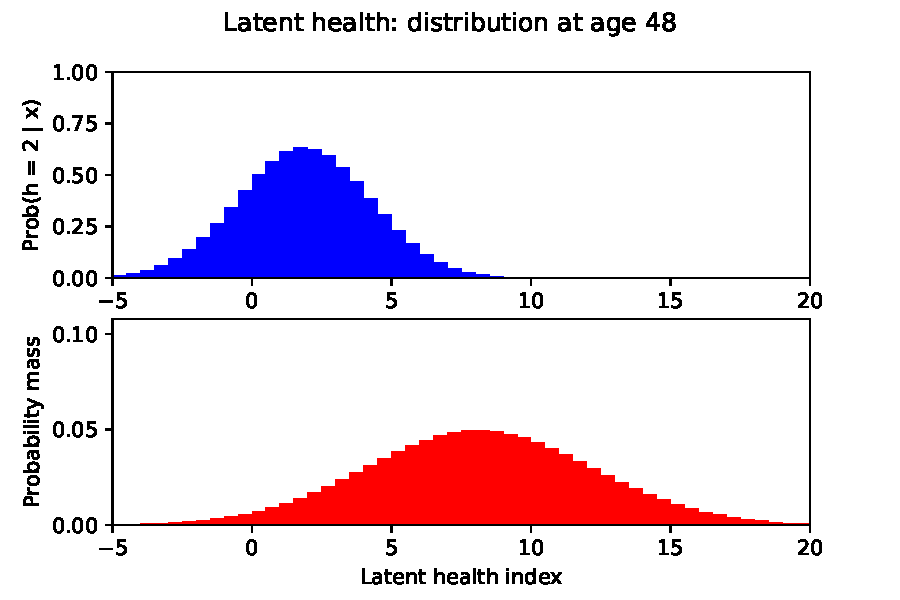
\includegraphics[scale=0.65]{\FigsDir/ReportDemo0.pdf}
\end{center}
\end{frame}

\begin{frame}\frametitle{Log likelihood function: self-reported health status}
\begin{center}
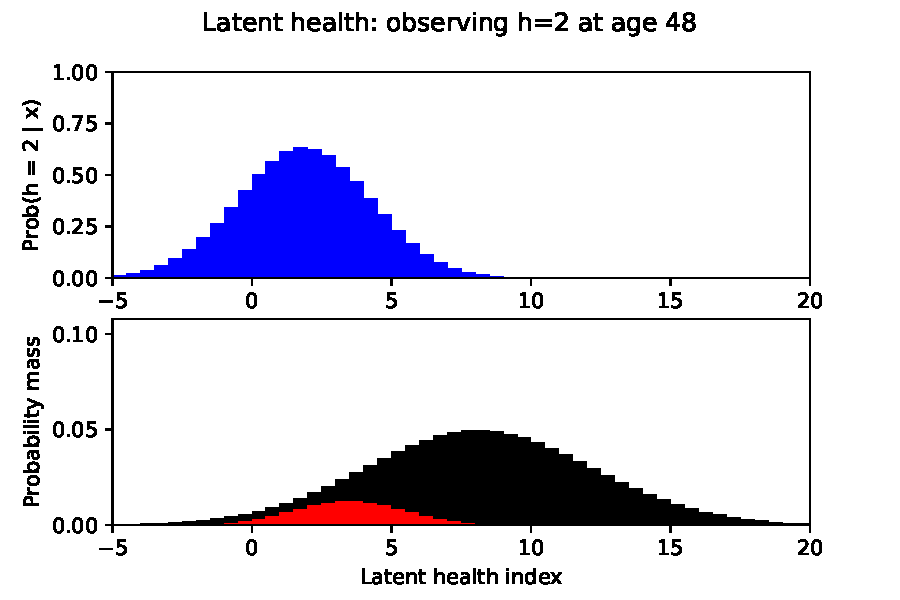
\includegraphics[scale=0.65]{\FigsDir/ReportDemo1.pdf}
\end{center}
\end{frame}

\begin{frame}\frametitle{Log likelihood function: self-reported health status}
\begin{center}
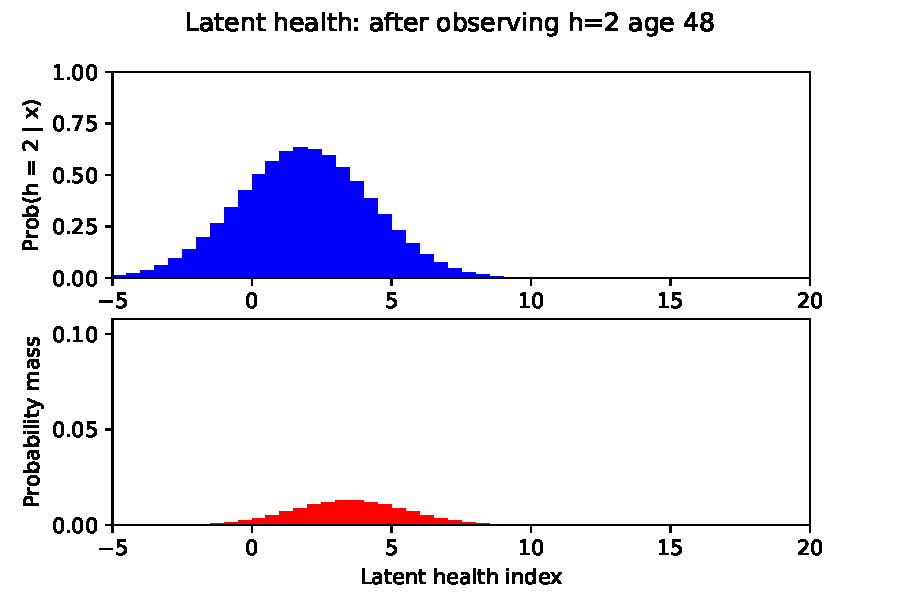
\includegraphics[scale=0.65]{\FigsDir/ReportDemo2.pdf}
\end{center}
\end{frame}

\begin{frame}\frametitle{Log likelihood function: self-reported health status}
\begin{center}
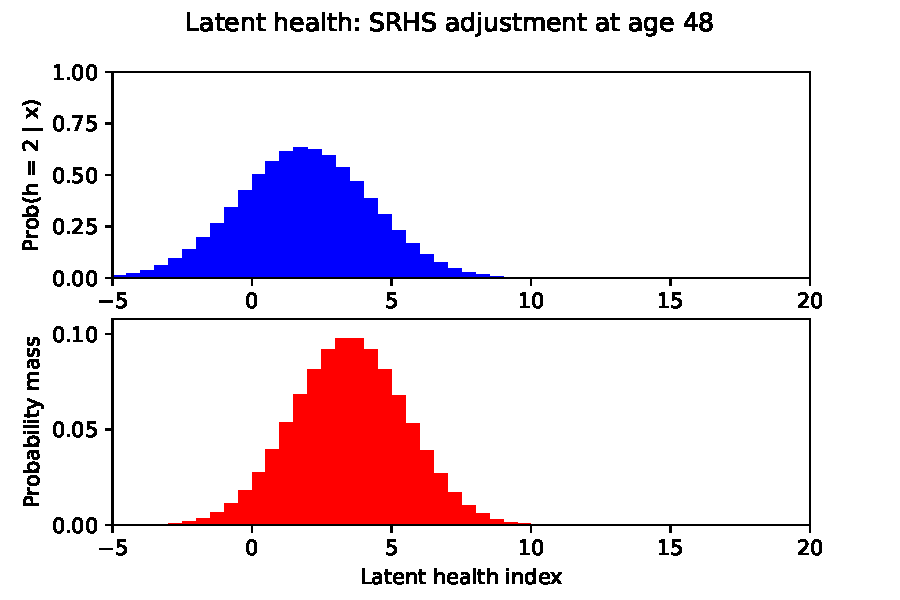
\includegraphics[scale=0.65]{\FigsDir/ReportDemo3.pdf}
\end{center}
\end{frame}


\begin{frame}\frametitle{Log likelihood function: mortality}
\begin{center}
	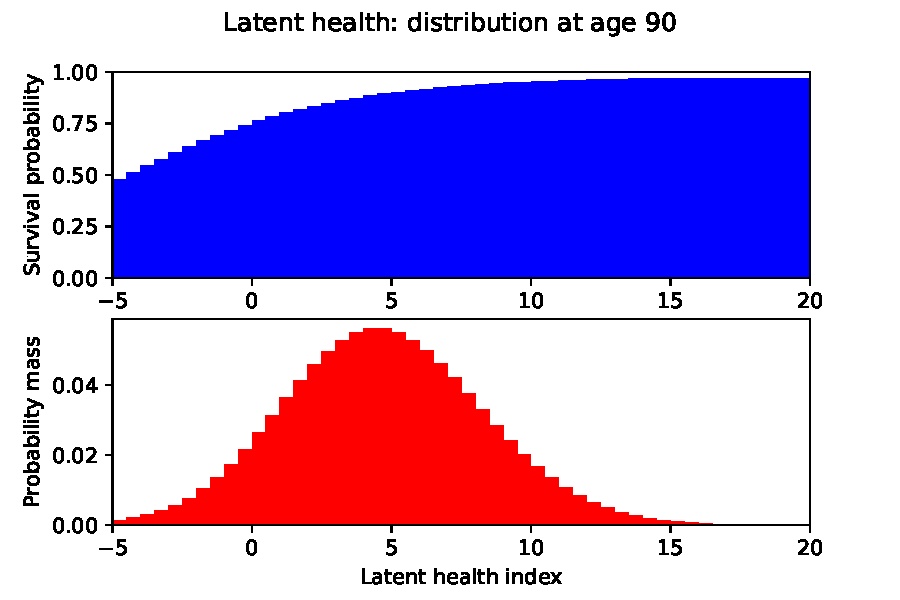
\includegraphics[scale=0.65]{\FigsDir/MortalityDemo0.pdf}
\end{center}
\end{frame}

\begin{frame}\frametitle{Log likelihood function: mortality}
\begin{center}
	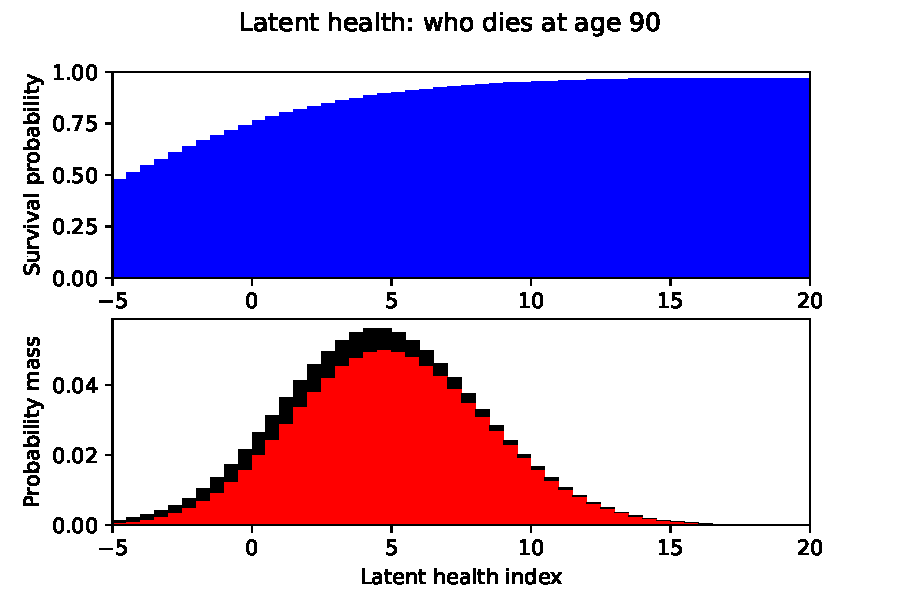
\includegraphics[scale=0.65]{\FigsDir/MortalityDemo1.pdf}
\end{center}
\end{frame}

\begin{frame}\frametitle{Log likelihood function: mortality}
\begin{center}
	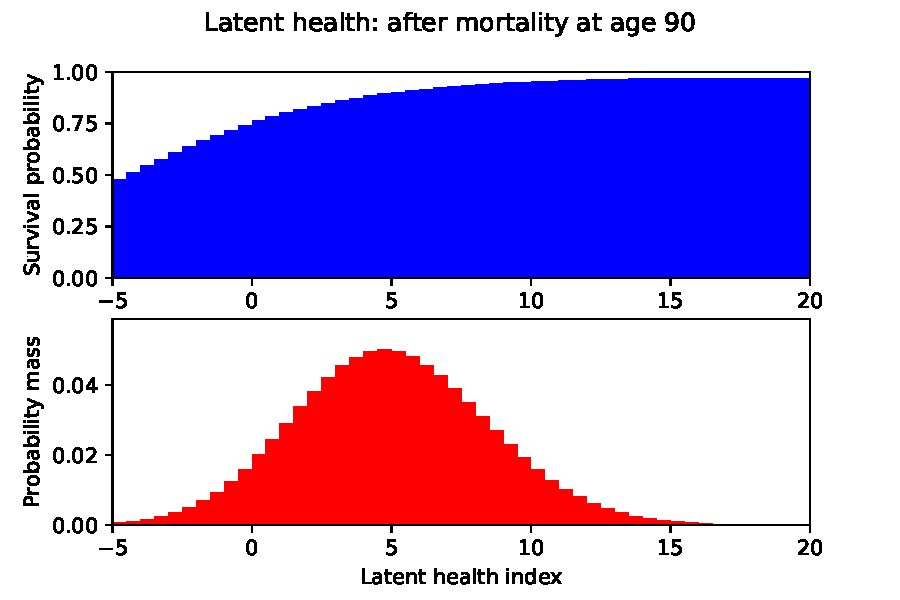
\includegraphics[scale=0.65]{\FigsDir/MortalityDemo2.pdf}
\end{center}
\end{frame}

\begin{frame}\frametitle{Log likelihood function: mortality}
\begin{center}
	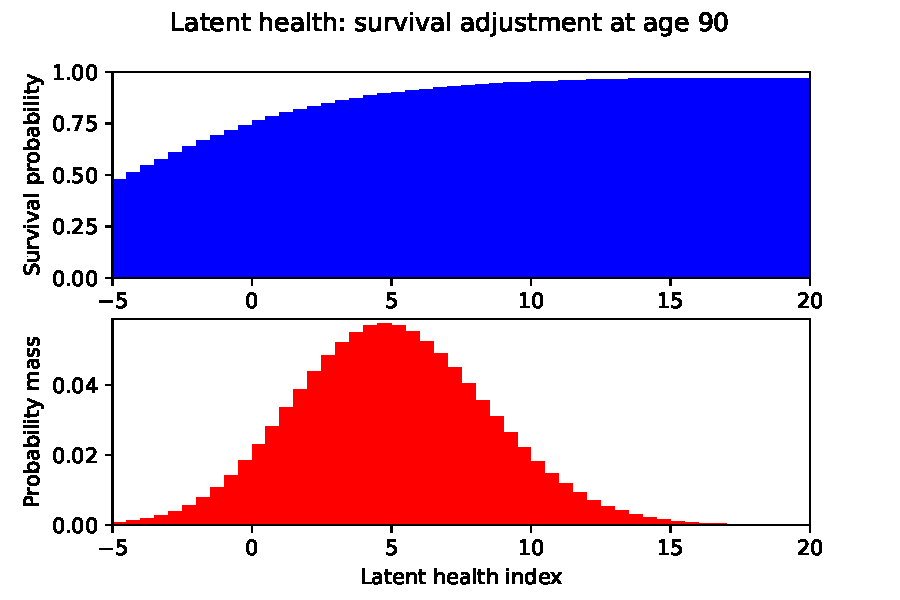
\includegraphics[scale=0.65]{\FigsDir/MortalityDemo3.pdf}
\end{center}
\end{frame}

\begin{frame}\frametitle{Log likelihood function: mortality}
\begin{center}
	\includegraphics[scale=0.65]{\FigsDir/MortalityDemo0.pdf}
\end{center}
\end{frame}


\begin{frame}\frametitle{Log likelihood function: latent health transitions}
\begin{center}
	\includegraphics[scale=0.65]{\FigsDir/HealthTransAnimation/FirstFrame.pdf}
\end{center}
\end{frame}

\begin{frame}\frametitle{Log likelihood function: latent health transitions}
\begin{center}
	\animategraphics[autoplay, scale=0.65]{3}{\FigsDir/HealthTransAnimation/frame}{0}{100}
\end{center}
\end{frame}

\begin{frame}\frametitle{Log likelihood function: latent health transitions}
\begin{center}
	\includegraphics[scale=0.65]{\FigsDir/HealthTransAnimation/LastFrame.pdf}
\end{center}
\end{frame}


\begin{frame}\frametitle{Identification challenge}
\begin{itemize}
	\item <1->$\alpha_1$ near zero means SRHS is mostly reporting error
	
	\item <1->High $\alpha_1$ means SRHS is almost perfect report of health
	
	\item <2->Holding $\rho_{j}$ fixed, lower $\alpha_1$ means SRHS changes more between $t$ and $t+1$
	
	\item <3->$\rho_{j}$ near zero means latent health is (almost) iid
	
	\item <3->$\rho_{j}$ near one means it's (almost) a random walk
	
	\item <4->Holding $\alpha_1$ fixed, lower $\rho_j$ means SRHS changes more between $t$ and $t+1$
	
	\item <5->How to tell apart low correlation in latent health from large reporting shocks?
\end{itemize}
\end{frame}


\begin{frame}\frametitle{Identification strategy (1/2)}
\begin{itemize}
	\item <1->How to tell apart low correlation in latent health from large reporting shocks?
	
	\item <2->Fit \textbf{sequences} of SRHS, not just transitions
	
	\item <2->Separate correlation of latent health from reporting error by $t$ to $t+n$ transitions
	
	\item <3->Compare SRHS of fair-to-poor R's vs fair-to-good R's in $t+2$
	
	\item <4->More similar distributions of SRHS: low $\alpha_1$, high $\rho_j$
	
	\item <4->Less similar distributions of SRHS: high $\alpha_1$, low $\rho_j$
	
	\item <5->Need more than 2 SRHS categories to do this!
\end{itemize}
\end{frame}


\begin{frame}\frametitle{Identification strategy (2/2)}
\begin{itemize}
	\item <1->Rest of the parameters are straightforward to identify
	
	\item <1->Main difficulty: Changing $\alpha_1$ and $\gamma$ parameters changes scale of $x_t$... requiring many other parameters to adjust!
	
	\item <2->Identify mortality params $\theta$ off of deaths by age and SRHS
	
	\item <3->Identify expected health parameters $\beta$, initial health distribution $(\mu_0, \sigma_0^2)$, and probit cut points $\chi$ from distribution of SRHS by age
\end{itemize}
\end{frame}


\section{Data \& Results}


\begin{frame}
\begin{center}
	\Huge
	DATA
\end{center}
\end{frame}


\subsection{Datasets}

\begin{frame}\frametitle{Medical Expenditure Panel Survey}
\begin{itemize}
\item <1->Began in 1996, focused on medical events \& expenses

\item <1->Nationally representative sample (weights provided)

\item <1->Short panel: respondents interviewed five times over 2 years

\item <1->New panel started every year (overlapping panels)

\item <2->Use Panels 1-20, spanning 1996-2017

\item <2->Drop under 18's and over 84's (age is topcoded at 85)

\item <2->Relabel age to have half-years based on age in W1 and W2

\item <3->126,486 women observed for 601,713 waves (1,168 deaths)

\item <3->110,044 men observed for 518,577 waves (1,314 deaths)

\item <3->89\% of respondents observed all 5 waves; most others drop after 3 (maybe planned drops?)

\end{itemize}
\end{frame}

\begin{frame}\frametitle{Health and Retirement Survey}
\begin{itemize}
\item <1->Begins ``in earnest'' in 1996-- oldest cohorts started in 1993

\item <1->Respondents enter around age 55; nationally representative

\item <1->Long panel: R's interviewed every two years (until death)

\item <2->Use 1996 to 2016 data waves (11 waves)

\item <2->Drop R's under 50's: not enough spouses this young

\item <2->Drop R's first observed older than age 95 (not enough)

\item <2->Observe SRHS every 2 years; recoded to 1 year periods

\item <3->20,108 women observed for 107,542 waves (5,794 deaths)

\item <3->16,094 men observed for 81,091 waves (5,286 deaths)

\item <3->50\% observed alive at least 5 waves, 11\% obs all 11 waves
\end{itemize}
\end{frame}

\begin{frame}\frametitle{Panel Study of Income Dynamics}
\begin{itemize}
\item <1->Began in 1968 with nationally representative sample of HH's

\item <1->Snowballing sample (with recent immigrants added)

\item <1->Long panel: annual interviews until 1997, biannual since

\item <2->Use data from 1997 to 2017 (11 waves, recode to 21 years)

\item <2->SRHS \textbf{only} asked of HH heads and spouses

\item <2->Selection bias: college students aren't heads yet!

\item <2->Enter my data at age 23; also drop R's who start 90+

\item <3->11,787 women observed for 69,329 waves (1,012 deaths)

\item <3->10,791 men observed for 58,316 waves (995 deaths)

\item <3->32\% observed 2 waves or fewer, but 22\% obs all 11 waves

\end{itemize}
\end{frame}


\subsection{Estimated model(s)}


\begin{frame}
\begin{center}
	\Huge
	RESULTS
\end{center}
\end{frame}


\begin{frame}\frametitle{Estimated parameters: MEPS women (mortality)}
\begin{table}[ht]\label{MEPSwomenMortParams}
\footnotesize
\begin{center}
\begin{tabular}{clc}
\hline \hline
Param & Description & MEPS \\
\hline
$\theta_{0}'$ & Mortality probit: level at model start $\underline{j}$ & 2.689 \\
 & & (2.85e-2) \\
$\theta_{h1}'$ & Mortality probit: first derivative w.r.t health at $\Health=0$ & 0.120 \\
 & & (7.24e-3) \\
$\theta_{h2}'$ & Mortality probit: second derivative w.r.t health at $\Health=0$ & 1.97e-2 \\
 & & (3.16e-3) \\
$\theta_{h3}'$ & Mortality probit: third derivative w.r.t health at $\Health=0$ & 1.01e-3 \\
 & & (3.68e-4) \\
$\theta_{j1}'$ & Mortality probit: first derivative w.r.t age at $\underline{j}$ & -6.14e-4 \\
 & & (2.06e-5) \\
$\theta_{j2}'$ & Mortality probit: second derivative w.r.t age at $\underline{j}$ & 5.76e-7 \\
 & & (2.63e-7) \\
$\theta_{j3}'$ & Mortality probit: third derivative w.r.t age at $\underline{j}$ & -9.88e-5 \\
 & & (3.66e-5) \\
\hline\hline
\end{tabular}
\end{center}
\end{table}

\end{frame}


\begin{frame}\frametitle{Model fit: Mortality by age for MEPS women}
\begin{center}
	\includegraphics[scale=0.65]{\FigsDir/MEPSover18WomenMortbyAge.pdf}
\end{center}
\end{frame}

\begin{frame}\frametitle{Model fit: Mortality by age and SRHS for MEPS women}
\begin{center}
	\includegraphics[scale=0.65]{\FigsDir/MEPSover18WomenMortbyAgeHealth.pdf}
\end{center}
\end{frame}


\begin{frame}\frametitle{Estimated parameters: MEPS women (latent health)}
\begin{table}[ht]\label{MEPSwomenHealthParams}
\footnotesize
\begin{center}
\begin{tabular}{clc}
\hline \hline
Param & Description & MEPS \\
\hline
$\gamma_{j3}'$ & Correlation factor: third derivative w.r.t age at $\underline{j}$ & 7.616 \\
 & & (0.100) \\
$\beta_{0}'$ & Expected health: level at model start $\underline{j}$ & 0.134 \\
 & & (1.90e-2) \\
$\beta_{j1}'$ & Expected health: first derivative w.r.t age at $\underline{j}$ & -2.68e-2 \\
 & & (2.56e-3) \\
$\beta_{j2}'$ & Expected health: second derivative w.r.t age at $\underline{j}$ & 2.02e-3 \\
 & & (1.91e-4) \\
$\beta_{j3}'$ & Expected health: third derivative w.r.t age at $\underline{j}$ & -6.67e-5 \\
 & & (6.29e-6) \\
$\beta_{j4}'$ & Expected health: fourth derivative w.r.t age at $\underline{j}$ & 9.402 \\
 & & (9.09e-2) \\
$\mu_0$ & Mean of latent health at $\underline{j}$ & 3.166 \\
 & & (4.51e-2) \\
\hline\hline
\end{tabular}
\end{center}
\end{table}

\end{frame}


\begin{frame}\frametitle{Estimated model: Distribution of latent health (MEPS women)}
\begin{center}
	\includegraphics[scale=0.65]{\FigsDir/MEPSover18HealthDstnWomen.pdf}
\end{center}
\end{frame}


\begin{frame}\frametitle{Estimated parameters: MEPS women (correlation and SRHS)}
\vspace{-0.25cm}
\begin{table}[ht]\label{MEPSwomenOtherParams}
\footnotesize
\begin{center}
\begin{tabular}{clc}
\hline \hline
Param & Description & MEPS \\
\hline
$\theta_{hj}$ & Mortality probit: coefficient on age$\times$health & 2.465 \\
 & & (2.77e-2) \\
$\gamma_{0}'$ & Correlation factor: level at model start $\underline{j}$ & 4.99e-2 \\
 & & (2.81e-3) \\
$\gamma_{j1}'$ & Correlation factor: first derivative w.r.t age at $\underline{j}$ & -1.82e-3 \\
 & & (2.00e-4) \\
$\gamma_{j2}'$ & Correlation factor: second derivative w.r.t age at $\underline{j}$ & 2.64e-5 \\
 & & (6.33e-6) \\
$\sigma_{0}$ & Standard deviation of latent health at $\underline{j}$ & 0.502 \\
 & & (5.37e-3) \\
$\alpha_1$ & SRHS: Linear coefficient on latent health & 1.597 \\
 & & (6.91e-3) \\
$\chi_2$ & SRHS: Cut b/w reporting ``fair'' and ``good'' & 3.389 \\
 & & (9.83e-3) \\
$\chi_3$ & SRHS: Cut b/w reporting ``good'' and ``very good'' & 5.111 \\
 & & (1.28e-2) \\
\hline\hline
\end{tabular}
\end{center}
\end{table}

\end{frame}


\begin{frame}\frametitle{Estimated model: Latent health serial correlation (MEPS women)}
\begin{center}
	\includegraphics[scale=0.65]{\FigsDir/MEPSover18WomenCorr.pdf}
\end{center}
\end{frame}


\begin{frame}\frametitle{Model fit: SRHS by age for MEPS women}
\begin{center}
	\includegraphics[scale=0.65]{\FigsDir/MEPSover18WomenSRHSbyAge.pdf}
\end{center}
\end{frame}


\begin{frame}\frametitle{Model fit: SRHS transitions for MEPS women: 1 wave}
\begin{center}
	\includegraphics[scale=0.65]{\FigsDir/MEPSover18WomenTransH5T1model.pdf}
\end{center}
\end{frame}

\begin{frame}\frametitle{Model fit: SRHS transitions for MEPS women: 1 wave}
\begin{center}
	\includegraphics[scale=0.65]{\FigsDir/MEPSover18WomenTransH4T1model.pdf}
\end{center}
\end{frame}

\begin{frame}\frametitle{Model fit: SRHS transitions for MEPS women: 1 wave}
\begin{center}
	\includegraphics[scale=0.65]{\FigsDir/MEPSover18WomenTransH3T1model.pdf}
\end{center}
\end{frame}

\begin{frame}\frametitle{Model fit: SRHS transitions for MEPS women: 1 wave}
\begin{center}
	\includegraphics[scale=0.65]{\FigsDir/MEPSover18WomenTransH2T1model.pdf}
\end{center}
\end{frame}

\begin{frame}\frametitle{Model fit: SRHS transitions for MEPS women: 1 wave}
\begin{center}
	\includegraphics[scale=0.65]{\FigsDir/MEPSover18WomenTransH1T1model.pdf}
\end{center}
\end{frame}

\begin{frame}\frametitle{Model fit: SRHS transitions for MEPS women: 2 waves}
\begin{center}
	\includegraphics[scale=0.65]{\FigsDir/MEPSover18WomenTransH5T2model.pdf}
\end{center}
\end{frame}

\begin{frame}\frametitle{Model fit: SRHS transitions for MEPS women: 2 waves}
\begin{center}
\includegraphics[scale=0.65]{\FigsDir/MEPSover18WomenTransH4T2model.pdf}
\end{center}
\end{frame}

\begin{frame}\frametitle{Model fit: SRHS transitions for MEPS women: 2 waves}
\begin{center}
\includegraphics[scale=0.65]{\FigsDir/MEPSover18WomenTransH3T2model.pdf}
\end{center}
\end{frame}

\begin{frame}\frametitle{Model fit: SRHS transitions for MEPS women: 2 waves}
\begin{center}
\includegraphics[scale=0.65]{\FigsDir/MEPSover18WomenTransH2T2model.pdf}
\end{center}
\end{frame}

\begin{frame}\frametitle{Model fit: SRHS transitions for MEPS women: 2 waves}
\begin{center}
\includegraphics[scale=0.65]{\FigsDir/MEPSover18WomenTransH1T2model.pdf}
\end{center}
\end{frame}

\begin{frame}\frametitle{Model fit: SRHS transitions for MEPS women: 4 waves}
\begin{center}
	\includegraphics[scale=0.65]{\FigsDir/MEPSover18WomenTransH5T4model.pdf}
\end{center}
\end{frame}

\begin{frame}\frametitle{Model fit: SRHS transitions for MEPS women: 4 waves}
\begin{center}
\includegraphics[scale=0.65]{\FigsDir/MEPSover18WomenTransH4T4model.pdf}
\end{center}
\end{frame}

\begin{frame}\frametitle{Model fit: SRHS transitions for MEPS women: 4 waves}
\begin{center}
\includegraphics[scale=0.65]{\FigsDir/MEPSover18WomenTransH3T4model.pdf}
\end{center}
\end{frame}

\begin{frame}\frametitle{Model fit: SRHS transitions for MEPS women: 4 waves}
\begin{center}
\includegraphics[scale=0.65]{\FigsDir/MEPSover18WomenTransH2T4model.pdf}
\end{center}
\end{frame}

\begin{frame}\frametitle{Model fit: SRHS transitions for MEPS women: 4 waves}
\begin{center}
\includegraphics[scale=0.65]{\FigsDir/MEPSover18WomenTransH1T4model.pdf}
\end{center}
\end{frame}

\begin{frame}\frametitle{Model fit: Duration dependence, ``healthy'' to ``unhealthy''}
\begin{center}
	\includegraphics[scale=0.65]{\FigsDir/MEPSover18WomenDurDepT1G2B.pdf}
\end{center}
\end{frame}

\begin{frame}\frametitle{Model fit: Duration dependence, ``healthy'' to ``unhealthy''}
\begin{center}
	\includegraphics[scale=0.65]{\FigsDir/MEPSover18WomenDurDepT2G2B.pdf}
\end{center}
\end{frame}

\begin{frame}\frametitle{Model fit: Duration dependence, ``healthy'' to ``unhealthy''}
\begin{center}
	\includegraphics[scale=0.65]{\FigsDir/MEPSover18WomenDurDepT3G2B.pdf}
\end{center}
\end{frame}

\begin{frame}\frametitle{Model fit: Duration dependence, ``healthy'' to ``unhealthy''}
\begin{center}
	\includegraphics[scale=0.65]{\FigsDir/MEPSover18WomenDurDepT4G2B.pdf}
\end{center}
\end{frame}

\begin{frame}\frametitle{Model fit: Duration dependence, ``unhealthy'' to ``healthy''}
\begin{center}
	\includegraphics[scale=0.65]{\FigsDir/MEPSover18WomenDurDepT1B2G.pdf}
\end{center}
\end{frame}

\begin{frame}\frametitle{Model fit: Duration dependence, ``unhealthy'' to ``healthy''}
\begin{center}
	\includegraphics[scale=0.65]{\FigsDir/MEPSover18WomenDurDepT2B2G.pdf}
\end{center}
\end{frame}

\begin{frame}\frametitle{Model fit: Duration dependence, ``unhealthy'' to ``healthy''}
\begin{center}
	\includegraphics[scale=0.65]{\FigsDir/MEPSover18WomenDurDepT3B2G.pdf}
\end{center}
\end{frame}

\begin{frame}\frametitle{Model fit: Duration dependence, ``unhealthy'' to ``healthy''}
\begin{center}
	\includegraphics[scale=0.65]{\FigsDir/MEPSover18WomenDurDepT4B2G.pdf}
\end{center}
\end{frame}


\begin{frame}\frametitle{Estimated model: Changing SRHS if asked twice (MEPS women)}
\begin{center}
	\includegraphics[scale=0.65]{\FigsDir/MEPSover18WomenChangeSRHS.pdf}
\end{center}
\end{frame}


\begin{frame}\frametitle{Estimated model: Predicting (log) medical expenses}
\begin{itemize}
\item <1->SRHS is known to be predictive of (log) medical costs

\item <1->How does model-predicted latent health $x_t$ do?

\item <2->For all 125 possible sequences of SRHS in waves 1-3 at each age, use estimated model to calculate $\hat{x}_t = \E[x_t]$ and $\widehat{x^2}_t = \E[x_t^2]$

\item <2->Get total medical expenses between waves 3 and 5 (1 year)

\item <3->Regress $\log(TotalMed)$ on cubic in age, $\hat{x}_t$, and $\widehat{x^2}_t$: $R^2 = 0.1600$

\item <3->Regress $\log(TotalMed)$ on \textbf{full interaction} of age and SRHS: $R^2 = 0.1602$

\item <4->Same exercise for men: $R^2 = 0.2326$ (latent health) vs $R^2 = 0.2326$ (full interact)
\end{itemize}
\end{frame}


\begin{frame}\frametitle{Estimated model: Out-of-sample fit}
\begin{itemize}
\item <1->Also estimated model on PSID and HRS, men and women; all fit well

\item <1->Model was estimated on \textbf{short panel} MEPS data and fit it well...

\item <1->...But does its long term predictions fit \textbf{long panel} datasets?

\item <2->PSID and HRS ask for SRHS every 2 years over same timeframe

\item <2->Can project estimated model out to see fit of 4-20 year ahead transitions

\item <3->Result: \textbf{No, it absolutely does not fit}

\item <4->Probably too much of a stretch to project a model 10x beyond data

\item <4->MEPS has a selection bias problem: too few respondents in poor health

\item <4->And asks respondents to compare to people of their own age
\end{itemize}
\end{frame}



\begin{frame}\frametitle{SRHS across datasets: MEPS, HRS, and PSID (women)}
\begin{center}
	\includegraphics[scale=0.65]{\FigsDir/CrossDataSRHSaWomen.pdf}
\end{center}
\end{frame}


\begin{frame}\frametitle{Cross-dataset sample construction}
\begin{itemize}
\item <1->Can fix two of those problems (but selection bias remains)

\item <2->Can create merged dataset across MEPS-SAQ, HRS, and PSID

\item <2->MEPS-SAQ: Mail-in supplemental survey that includes SRHS (waves 2 \& 4)

\item <2->Use 1 year periods for model: 1 period transitions only seen in MEPS!

\item <3->Short run transitions from MEPS, long run paths from HRS \& PSID

\item <3->Model starts at age 18; drop R's who start over age 90 (84 for MEPS)

\item <3->Only admit PSID respondents when they turn 23

\item <4->120,055 women observed for 342,796 waves (6,918 deaths)

\item <4->102,965 men observed for 281,681 waves (6,568 deaths)

\item <4->82\% of respondents observed 2 or fewer waves (mostly MEPS)
\end{itemize}
\end{frame}


\begin{frame}\frametitle{SRHS across datasets: MEPS-SAQ, HRS, and PSID (women)}
\begin{center}
	\includegraphics[scale=0.65]{\FigsDir/CrossDataSRHSbWomen.pdf}
\end{center}
\end{frame}

\begin{frame}\frametitle{SRHS across datasets: MEPS, HRS, and PSID (women)}
\begin{center}
	\includegraphics[scale=0.65]{\FigsDir/CrossDataSRHSaWomen.pdf}
\end{center}
\end{frame}



\begin{frame}\frametitle{Naive SRHS transitions for cross-data women: 1 year}
\begin{center}
	\includegraphics[scale=0.65]{\FigsDir/CrossDataWomenTransH5T1naive.pdf}
\end{center}
\end{frame}

\begin{frame}\frametitle{Naive SRHS transitions for cross-data women: 1 year}
\begin{center}
	\includegraphics[scale=0.65]{\FigsDir/CrossDataWomenTransH4T1naive.pdf}
\end{center}
\end{frame}

\begin{frame}\frametitle{Naive SRHS transitions for cross-data women: 1 year}
\begin{center}
	\includegraphics[scale=0.65]{\FigsDir/CrossDataWomenTransH3T1naive.pdf}
\end{center}
\end{frame}

\begin{frame}\frametitle{Naive SRHS transitions for cross-data women: 1 year}
\begin{center}
	\includegraphics[scale=0.65]{\FigsDir/CrossDataWomenTransH2T1naive.pdf}
\end{center}
\end{frame}

\begin{frame}\frametitle{Naive SRHS transitions for cross-data women: 1 year}
\begin{center}
	\includegraphics[scale=0.65]{\FigsDir/CrossDataWomenTransH1T1naive.pdf}
\end{center}
\end{frame}

\begin{frame}\frametitle{Naive SRHS transitions for cross-data women: 2 years}
\begin{center}
	\includegraphics[scale=0.65]{\FigsDir/CrossDataWomenTransH5T2naive.pdf}
\end{center}
\end{frame}

\begin{frame}\frametitle{Naive SRHS transitions for cross-data women: 2 years}
\begin{center}
\includegraphics[scale=0.65]{\FigsDir/CrossDataWomenTransH4T2naive.pdf}
\end{center}
\end{frame}

\begin{frame}\frametitle{Naive SRHS transitions for cross-data women: 2 years}
\begin{center}
\includegraphics[scale=0.65]{\FigsDir/CrossDataWomenTransH3T2naive.pdf}
\end{center}
\end{frame}

\begin{frame}\frametitle{Naive SRHS transitions for cross-data women: 2 years}
\begin{center}
\includegraphics[scale=0.65]{\FigsDir/CrossDataWomenTransH2T2naive.pdf}
\end{center}
\end{frame}

\begin{frame}\frametitle{Naive SRHS transitions for cross-data women: 2 years}
\begin{center}
\includegraphics[scale=0.65]{\FigsDir/CrossDataWomenTransH1T2naive.pdf}
\end{center}
\end{frame}

\begin{frame}\frametitle{Naive SRHS transitions for cross-data women: 10 years}
\begin{center}
	\includegraphics[scale=0.65]{\FigsDir/CrossDataWomenTransH5T10naive.pdf}
\end{center}
\end{frame}

\begin{frame}\frametitle{Naive SRHS transitions for cross-data women: 10 years}
\begin{center}
\includegraphics[scale=0.65]{\FigsDir/CrossDataWomenTransH4T10naive.pdf}
\end{center}
\end{frame}

\begin{frame}\frametitle{Naive SRHS transitions for cross-data women: 10 years}
\begin{center}
\includegraphics[scale=0.65]{\FigsDir/CrossDataWomenTransH3T10naive.pdf}
\end{center}
\end{frame}

\begin{frame}\frametitle{Naive SRHS transitions for cross-data women: 10 years}
\begin{center}
\includegraphics[scale=0.65]{\FigsDir/CrossDataWomenTransH2T10naive.pdf}
\end{center}
\end{frame}

\begin{frame}\frametitle{Naive SRHS transitions for cross-data women: 10 years}
\begin{center}
\includegraphics[scale=0.65]{\FigsDir/CrossDataWomenTransH1T10naive.pdf}
\end{center}
\end{frame}


\begin{frame}\frametitle{Estimated parameters: Cross-data women (mortality)}
\begin{table}[ht]\label{CrossWomenMortParams}
\footnotesize
\begin{center}
\begin{tabular}{clc}
\hline \hline
Param & Description & Cross \\
\hline
$\theta_{0}'$ & Mortality probit: level at model start $\underline{j}$ & 2.793 \\
 & & (0.111) \\
$\theta_{h1}'$ & Mortality probit: first derivative w.r.t health at $\Health=0$ & 0.127 \\
 & & (7.24e-3) \\
$\theta_{h2}'$ & Mortality probit: second derivative w.r.t health at $\Health=0$ & 5.85e-3 \\
 & & (1.72e-3) \\
$\theta_{h3}'$ & Mortality probit: third derivative w.r.t health at $\Health=0$ & -3.21e-2 \\
 & & (7.30e-3) \\
$\theta_{j1}'$ & Mortality probit: first derivative w.r.t age at $\underline{j}$ & 1.08e-3 \\
 & & (3.22e-4) \\
$\theta_{j2}'$ & Mortality probit: second derivative w.r.t age at $\underline{j}$ & -4.21e-5 \\
 & & (6.85e-6) \\
$\theta_{j3}'$ & Mortality probit: third derivative w.r.t age at $\underline{j}$ & -1.81e-4 \\
 & & (8.17e-5) \\
\hline\hline
\end{tabular}
\end{center}
\end{table}

\end{frame}


\begin{frame}\frametitle{Model fit: Mortality by age for cross-data women}
\begin{center}
\includegraphics[scale=0.65]{\FigsDir/CrossDataWomenMortbyAge.pdf}
\end{center}
\end{frame}


\begin{frame}\frametitle{Model fit: Mortality by age-SRHS for cross-data women}
\begin{center}
\includegraphics[scale=0.65]{\FigsDir/CrossDataWomenMortbyAgeHealth.pdf}
\end{center}
\end{frame}


\begin{frame}\frametitle{Estimated parameters: Cross-data women (health)}
\begin{table}[ht]\label{CrossWomenHealthParams}
\footnotesize
\begin{center}
\begin{tabular}{clc}
\hline \hline
Param & Description & Cross \\
\hline
$\gamma_{j3}'$ & Correlation factor: third derivative w.r.t age at $\underline{j}$ & 10.812 \\
 & & (0.230) \\
$\beta_{0}'$ & Expected health: level at model start $\underline{j}$ & -0.341 \\
 & & (2.93e-2) \\
$\beta_{j1}'$ & Expected health: first derivative w.r.t age at $\underline{j}$ & 6.01e-3 \\
 & & (2.79e-3) \\
$\beta_{j2}'$ & Expected health: second derivative w.r.t age at $\underline{j}$ & 7.73e-4 \\
 & & (2.21e-4) \\
$\beta_{j3}'$ & Expected health: third derivative w.r.t age at $\underline{j}$ & -5.54e-5 \\
 & & (8.65e-6) \\
$\beta_{j4}'$ & Expected health: fourth derivative w.r.t age at $\underline{j}$ & 9.995 \\
 & & (0.118) \\
$\mu_0$ & Mean of latent health at $\underline{j}$ & 3.607 \\
 & & (6.96e-2) \\
\hline\hline
\end{tabular}
\end{center}
\end{table}

\end{frame}


\begin{frame}\frametitle{Estimated model: Distribution of latent health (cross-data women)}
\begin{center}
	\includegraphics[scale=0.65]{\FigsDir/CrossDataHealthDstnWomen.pdf}
\end{center}
\end{frame}


\begin{frame}\frametitle{Estimated parameters: Cross-data women (correlation and SRHS)}
\vspace{-0.25cm}
\begin{table}[ht]\label{CrossWomenOtherParams}
\footnotesize
\begin{center}
\begin{tabular}{clc}
\hline \hline
Param & Description & Cross \\
\hline
$\theta_{hj}$ & Mortality probit: coefficient on age$\times$health & 2.622 \\
 & & (5.47e-2) \\
$\gamma_{0}'$ & Correlation factor: level at model start $\underline{j}$ & 9.28e-2 \\
 & & (6.14e-3) \\
$\gamma_{j1}'$ & Correlation factor: first derivative w.r.t age at $\underline{j}$ & -5.03e-3 \\
 & & (3.92e-4) \\
$\gamma_{j2}'$ & Correlation factor: second derivative w.r.t age at $\underline{j}$ & 1.21e-4 \\
 & & (1.10e-5) \\
$\sigma_{0}$ & Standard deviation of latent health at $\underline{j}$ & 0.472 \\
 & & (5.59e-3) \\
$\alpha_1$ & SRHS: Linear coefficient on latent health & 1.802 \\
 & & (9.76e-3) \\
$\chi_2$ & SRHS: Cut b/w reporting ``fair'' and ``good'' & 3.802 \\
 & & (1.46e-2) \\
$\chi_3$ & SRHS: Cut b/w reporting ``good'' and ``very good'' & 5.954 \\
 & & (2.01e-2) \\
\hline\hline
\end{tabular}
\end{center}
\end{table}

\end{frame}


\begin{frame}\frametitle{Estimated model: Latent health serial correlation (cross-dataset women)}
\begin{center}
	\includegraphics[scale=0.65]{\FigsDir/CrossDataWomenCorr.pdf}
\end{center}
\end{frame}


\begin{frame}\frametitle{Model fit: SRHS by age for cross-data women}
\begin{center}
	\includegraphics[scale=0.65]{\FigsDir/CrossDataWomenSRHSbyAge.pdf}
\end{center}
\end{frame}


\begin{frame}\frametitle{Model fit: SRHS transitions for cross-data women: 1 year}
\begin{center}
	\includegraphics[scale=0.65]{\FigsDir/CrossDataWomenTransH5T1model.pdf}
\end{center}
\end{frame}

\begin{frame}\frametitle{Model fit: SRHS transitions for cross-data women: 1 year}
\begin{center}
\includegraphics[scale=0.65]{\FigsDir/CrossDataWomenTransH4T1model.pdf}
\end{center}
\end{frame}

\begin{frame}\frametitle{Model fit:e SRHS transitions for cross-data women: 1 year}
\begin{center}
\includegraphics[scale=0.65]{\FigsDir/CrossDataWomenTransH3T1model.pdf}
\end{center}
\end{frame}

\begin{frame}\frametitle{Model fit: SRHS transitions for cross-data women: 1 year}
\begin{center}
\includegraphics[scale=0.65]{\FigsDir/CrossDataWomenTransH2T1model.pdf}
\end{center}
\end{frame}

\begin{frame}\frametitle{Model fit: SRHS transitions for cross-data women: 1 year}
\begin{center}
\includegraphics[scale=0.65]{\FigsDir/CrossDataWomenTransH1T1model.pdf}
\end{center}
\end{frame}

\begin{frame}\frametitle{Model fit: SRHS transitions for cross-data women: 2 years}
\begin{center}
\includegraphics[scale=0.65]{\FigsDir/CrossDataWomenTransH5T2model.pdf}
\end{center}
\end{frame}

\begin{frame}\frametitle{Model fit: SRHS transitions for cross-data women: 2 years}
\begin{center}
\includegraphics[scale=0.65]{\FigsDir/CrossDataWomenTransH4T2model.pdf}
\end{center}
\end{frame}

\begin{frame}\frametitle{Model fit: SRHS transitions for cross-data women: 2 years}
\begin{center}
\includegraphics[scale=0.65]{\FigsDir/CrossDataWomenTransH3T2model.pdf}
\end{center}
\end{frame}

\begin{frame}\frametitle{Model fit: SRHS transitions for cross-data women: 2 years}
\begin{center}
\includegraphics[scale=0.65]{\FigsDir/CrossDataWomenTransH2T2model.pdf}
\end{center}
\end{frame}

\begin{frame}\frametitle{Model fit: SRHS transitions for cross-data women: 2 years}
\begin{center}
\includegraphics[scale=0.65]{\FigsDir/CrossDataWomenTransH1T2model.pdf}
\end{center}
\end{frame}

\begin{frame}\frametitle{Model fit: SRHS transitions for cross-data women: 10 yrs}
\begin{center}
\includegraphics[scale=0.65]{\FigsDir/CrossDataWomenTransH5T10model.pdf}
\end{center}
\end{frame}

\begin{frame}\frametitle{Model fit: SRHS transitions for cross-data women: 10 yrs}
\begin{center}
\includegraphics[scale=0.65]{\FigsDir/CrossDataWomenTransH4T10model.pdf}
\end{center}
\end{frame}

\begin{frame}\frametitle{Model fit: SRHS transitions for cross-data women: 10 yrs}
\begin{center}
\includegraphics[scale=0.65]{\FigsDir/CrossDataWomenTransH3T10model.pdf}
\end{center}
\end{frame}

\begin{frame}\frametitle{Model fit: SRHS transitions for cross-data women: 10 yrs}
\begin{center}
\includegraphics[scale=0.65]{\FigsDir/CrossDataWomenTransH2T10model.pdf}
\end{center}
\end{frame}

\begin{frame}\frametitle{Model fit: SRHS transitions for cross-data women: 10 yrs}
\begin{center}
\includegraphics[scale=0.65]{\FigsDir/CrossDataWomenTransH1T10model.pdf}
\end{center}
\end{frame}

\begin{frame}\frametitle{Model fit: SRHS transitions for cross-data women: 1 year}
\begin{center}
	\includegraphics[scale=0.65]{\FigsDir/CrossDataWomenTransH3T1model.pdf}
\end{center}
\end{frame}

\begin{frame}\frametitle{Model fit: SRHS transitions for cross-data women: 2 years}
\begin{center}
	\includegraphics[scale=0.65]{\FigsDir/CrossDataWomenTransH3T2model.pdf}
\end{center}
\end{frame}

\begin{frame}\frametitle{Model fit: SRHS transitions for cross-data women: 4 years}
\begin{center}
	\includegraphics[scale=0.65]{\FigsDir/CrossDataWomenTransH3T4model.pdf}
\end{center}
\end{frame}

\begin{frame}\frametitle{Model fit: SRHS transitions for cross-data women: 6 years}
\begin{center}
	\includegraphics[scale=0.65]{\FigsDir/CrossDataWomenTransH3T6model.pdf}
\end{center}
\end{frame}

\begin{frame}\frametitle{Model fit: SRHS transitions for cross-data women: 8 years}
\begin{center}
	\includegraphics[scale=0.65]{\FigsDir/CrossDataWomenTransH3T8model.pdf}
\end{center}
\end{frame}

\begin{frame}\frametitle{Model fit: SRHS transitions for cross-data women: 10 yrs}
\begin{center}
	\includegraphics[scale=0.65]{\FigsDir/CrossDataWomenTransH3T10model.pdf}
\end{center}
\end{frame}

\begin{frame}\frametitle{Model fit: SRHS transitions for cross-data women: 12 yrs}
\begin{center}
	\includegraphics[scale=0.65]{\FigsDir/CrossDataWomenTransH3T12model.pdf}
\end{center}
\end{frame}

\begin{frame}\frametitle{Model fit: SRHS transitions for cross-data women: 14 yrs}
\begin{center}
	\includegraphics[scale=0.65]{\FigsDir/CrossDataWomenTransH3T14model.pdf}
\end{center}
\end{frame}

\begin{frame}\frametitle{Model fit: SRHS transitions for cross-data women: 16 yrs}
\begin{center}
	\includegraphics[scale=0.65]{\FigsDir/CrossDataWomenTransH3T16model.pdf}
\end{center}
\end{frame}

\begin{frame}\frametitle{Model fit: SRHS transitions for cross-data women: 18 yrs}
\begin{center}
	\includegraphics[scale=0.65]{\FigsDir/CrossDataWomenTransH3T18model.pdf}
\end{center}
\end{frame}

\begin{frame}\frametitle{Model fit: SRHS transitions for cross-data women: 20 yrs}
\begin{center}
	\includegraphics[scale=0.65]{\FigsDir/CrossDataWomenTransH3T20model.pdf}
\end{center}
\end{frame}

\begin{frame}\frametitle{Model fit: Duration dependence, ``healthy'' to ``unhealthy''}
\begin{center}
	\includegraphics[scale=0.65]{\FigsDir/CrossDataWomenDurDepT1G2B.pdf}
\end{center}
\end{frame}

\begin{frame}\frametitle{Model fit: Duration dependence, ``healthy'' to ``unhealthy''}
\begin{center}
	\includegraphics[scale=0.65]{\FigsDir/CrossDataWomenDurDepT2G2B.pdf}
\end{center}
\end{frame}

\begin{frame}\frametitle{Model fit: Duration dependence, ``healthy'' to ``unhealthy''}
\begin{center}
	\includegraphics[scale=0.65]{\FigsDir/CrossDataWomenDurDepT3G2B.pdf}
\end{center}
\end{frame}

\begin{frame}\frametitle{Model fit: Duration dependence, ``healthy'' to ``unhealthy''}
\begin{center}
	\includegraphics[scale=0.65]{\FigsDir/CrossDataWomenDurDepT4G2B.pdf}
\end{center}
\end{frame}

\begin{frame}\frametitle{Model fit: Duration dependence, ``unhealthy'' to ``healthy''}
\begin{center}
	\includegraphics[scale=0.65]{\FigsDir/CrossDataWomenDurDepT1B2G.pdf}
\end{center}
\end{frame}

\begin{frame}\frametitle{Model fit: Duration dependence, ``unhealthy'' to ``healthy''}
\begin{center}
	\includegraphics[scale=0.65]{\FigsDir/CrossDataWomenDurDepT2B2G.pdf}
\end{center}
\end{frame}

\begin{frame}\frametitle{Model fit: Duration dependence, ``unhealthy'' to ``healthy''}
\begin{center}
	\includegraphics[scale=0.65]{\FigsDir/CrossDataWomenDurDepT3B2G.pdf}
\end{center}
\end{frame}

\begin{frame}\frametitle{Model fit: Duration dependence, ``unhealthy'' to ``healthy''}
\begin{center}
\includegraphics[scale=0.65]{\FigsDir/CrossDataWomenDurDepT4B2G.pdf}
\end{center}
\end{frame}

\begin{frame}\frametitle{Estimated model: Changing SRHS if asked twice (cross-data women)}
\begin{center}
	\includegraphics[scale=0.65]{\FigsDir/CrossDataWomenChangeSRHS.pdf}
\end{center}
\end{frame}


\begin{frame}\frametitle{Model fit: Within-person distribution of ``unhealthy'' periods}
\begin{itemize}
\item DeNardi et al (2018) show that their duration dependence / unobserved heterogeneity model fits the distribution of ``unhealthy'' periods over next 5 waves

\item Can the latent health model do that as well?
\end{itemize}
\begin{center}
	\includegraphics[scale=0.30]{\FigsDir/PPandDeNardiC.png}
\end{center}
\end{frame}


\begin{frame}\frametitle{Model fit: Freqency of reporting ``unhealthy'' (cross-data women)}
\begin{center}
	\includegraphics[scale=0.65]{\FigsDir/CrossDataWomenSRHSfreqH25to34.pdf}
\end{center}
\end{frame}

\begin{frame}\frametitle{Model fit: Freqency of reporting ``unhealthy'' (cross-data women)}
\begin{center}
	\includegraphics[scale=0.65]{\FigsDir/CrossDataWomenSRHSfreqH35to44.pdf}
\end{center}
\end{frame}

\begin{frame}\frametitle{Model fit: Freqency of reporting ``unhealthy'' (cross-data women)}
\begin{center}
	\includegraphics[scale=0.65]{\FigsDir/CrossDataWomenSRHSfreqH45to54.pdf}
\end{center}
\end{frame}

\begin{frame}\frametitle{Model fit: Freqency of reporting ``unhealthy'' (cross-data women)}
\begin{center}
	\includegraphics[scale=0.65]{\FigsDir/CrossDataWomenSRHSfreqH55to64.pdf}
\end{center}
\end{frame}

\begin{frame}\frametitle{Model fit: Freqency of reporting ``unhealthy'' (cross-data women)}
\begin{center}
	\includegraphics[scale=0.65]{\FigsDir/CrossDataWomenSRHSfreqH65to74.pdf}
\end{center}
\end{frame}

\begin{frame}\frametitle{Model fit: Freqency of reporting ``unhealthy'' (cross-data women)}
\begin{center}
	\includegraphics[scale=0.65]{\FigsDir/CrossDataWomenSRHSfreqH75to84.pdf}
\end{center}
\end{frame}

\begin{frame}\frametitle{Model fit: Freqency of reporting ``unhealthy'' (cross-data women)}
\begin{center}
	\includegraphics[scale=0.65]{\FigsDir/CrossDataWomenSRHSfreqU25to34.pdf}
\end{center}
\end{frame}

\begin{frame}\frametitle{Model fit: Freqency of reporting ``unhealthy'' (cross-data women)}
\begin{center}
\includegraphics[scale=0.65]{\FigsDir/CrossDataWomenSRHSfreqU35to44.pdf}
\end{center}
\end{frame}

\begin{frame}\frametitle{Model fit: Freqency of reporting ``unhealthy'' (cross-data women)}
\begin{center}
\includegraphics[scale=0.65]{\FigsDir/CrossDataWomenSRHSfreqU45to54.pdf}
\end{center}
\end{frame}

\begin{frame}\frametitle{Model fit: Freqency of reporting ``unhealthy'' (cross-data women)}
\begin{center}
\includegraphics[scale=0.65]{\FigsDir/CrossDataWomenSRHSfreqU55to64.pdf}
\end{center}
\end{frame}

\begin{frame}\frametitle{Model fit: Freqency of reporting ``unhealthy'' (cross-data women)}
\begin{center}
\includegraphics[scale=0.65]{\FigsDir/CrossDataWomenSRHSfreqU65to74.pdf}
\end{center}
\end{frame}

\begin{frame}\frametitle{Model fit: Freqency of reporting ``unhealthy'' (cross-data women)}
\begin{center}
\includegraphics[scale=0.65]{\FigsDir/CrossDataWomenSRHSfreqU75to84.pdf}
\end{center}
\end{frame}


\subsection{Model extensions}


\begin{frame}
\begin{center}
	\Huge
	EXTENSIONS
\end{center}
\end{frame}


\begin{frame}\frametitle{Other work on latent health}
\begin{itemize}
	\item <1->Modeling health as a latent variable is not novel; long history
	
	\item <1->Actually new: estimating latent health dynamics on SRHS sequences
	
	\item <2->Lange \& McKee (2012): Use \textbf{multiple measures} to construct latent health index, estimate dynamics in second step
	
	\item <3->That still interprets measurement error as true change in health!
	
	\item <4->Blundell et al (2017): Investigate whether estimates of SRHS effect on retirement has self-justification bias (``I stopped working, so I must be unhealthy'')
	
	\item <5->No: Similar results with SRHS or constructed index from multiple measures.  Self-justification bias is offset by attenuation bias!
\end{itemize}
\end{frame}


\begin{frame}\frametitle{Improving my latent health model (1/2)}
\begin{itemize}
	\item <1->Why can't my model fit fraction of people who \textbf{consistently} report bad health?
	
	\item <1->Why does model have more switching between good and fair health than the data?
	
	\item <2->\textbf{Health types:} Some people don't recover from bad health because they have different transition probabilities
		
	\item <3->\textbf{SRHS subjectivity:} Some people have lower standard for what constitutes ``bad'' health, so they report bad health a lot (shift in $\chi$)
		
	\item <4->\textbf{Skewed health shocks:} Model assumes normal shocks to $x_t$, but left skewed shock distribution would put some people ``deeper'' into bad health
	
	\item <5->\textbf{Second latent factor:} One factor model is insufficient; second dimension of latent health is required to accurately represent dynamics
	
	\item <6->Which of these hypotheses can my model address with extensions?
\end{itemize}
\end{frame}


\begin{frame}\frametitle{Improving my latent health model (2/2)}
\begin{itemize}
	\item <1->Which of these hypotheses can model address with extensions? \textbf{ALL OF THEM}
	
	\item <1->Which of them \textbf{should} we look at first (or last)?
	
	\item <2->Unobserved heterogeneity in health process should be the explanation of last resort
	
	\item <3->MLE can handle second latent factor, but would be computationally expensive
	
	\item <3->And want representation of health that structural models can handle!
	
	\item <4->Need multiple measures to be able to address subjective SRHS, skewed shocks, or second latent factor, so let's start there
\end{itemize}
\end{frame}


\begin{frame}\frametitle{Other measures of health}
\begin{itemize}
	\item <1->Limitations on work, housework, or schoolwork due to health?
	
	\item <2->Activities of daily living: climbing stairs, carrying grocery bag
	
	\item <3->Mental health: How often feel nervous, hopeless, worthless, etc?
	
	\item <4->Extent to which pain interferes with normal work activities
	
	\item <5->Clinical measures: hand grip strength, walking speed, lung capacity
\end{itemize}
\end{frame}


\begin{frame}\frametitle{Latent health model with single measure (SRHS)}
Baseline latent health model:
\setcounter{equation}{0}
\begin{equation}
x_0 \sim N(\mu_0, \sigma^2_0).
\end{equation}

\begin{equation}
\Prob(h_{t+1} = 0) = 1 - \Phi(f(j_t,x_t)).
\end{equation}

\begin{equation}
x_{t+1} = \rho_{j} x_t + (1-\rho_j)g(j_t) + \epsilon_{t+1}, \qquad \epsilon_{t+1} \sim \Phi.
\end{equation}

\begin{equation}
h^*_t = \alpha_0 + \alpha_1 x_t + \eta_t, \qquad \eta_t \sim \Phi,
\end{equation}
\begin{equation*}
h_t = 1 + \sum_{k = 1}^{K-1} \mathbf{1}(h^*_t \geq \chi_k). 
\end{equation*}
\end{frame}


\begin{frame}\frametitle{Latent health model with multiple measures (1/2)}
Latent health model with multiple independent measures:
\setcounter{equation}{0}
\begin{equation}
x_0 \sim N(\mu_0, \sigma^2_0).
\end{equation}

\begin{equation}
\Prob(h_{t+1} = 0) = 1 - \Phi(f(j_t,x_t)).
\end{equation}

\begin{equation}
x_{t+1} = \rho_{j} x_t + (1-\rho_j)g(j_t) + \epsilon_{t+1}, \qquad \epsilon_{t+1} \sim \Phi.
\end{equation}

\begin{equation}
m^*_{\ell t} = \alpha_{\ell 0} + \alpha_{\ell 1} x_t + \eta_{\ell t}, \qquad \eta_{\ell t} \sim \Phi,
\end{equation}
\begin{equation*}
m_{\ell t} = 1 + \sum_{k = 1}^{K_{\ell}-1} \mathbf{1}(m^*_t \geq \chi_{k\ell}), \qquad \ell \in \{0,\cdots,L\}, \qquad h_t \equiv m_{0t}.
\end{equation*}
\end{frame}


\begin{frame}\frametitle{Latent health model with multiple measures (2/2)}
\begin{itemize}
	\item <1->Each wave, observe multiple categorical measures of latent health
	
	\item <1->Measure 0 is set aside for SRHS (and mortality)
	
	\item <1->Location assumption: $\chi_{1\ell} = 0 ~ \forall \ell$, but only $\alpha_{00} = 0$
	
	\item <2->Identifying assumption: Independence of reporting errors $\eta_{\ell t}$
	
	\item <2->Adding another measure \textbf{should not} affect estimates of other $\alpha$ coefficients
	
	\item <3->Obvious violation: Second latent factor (omitted variable bias)
	
	\item <4->My MLE code is already set up to estimate such a model, and appropriate datasets have been constructed...
	
	\item <4->...but I don't have a specification or results I'd like to share today
\end{itemize}
\end{frame}


\begin{frame}\frametitle{Adding other model extensions}
\begin{itemize}
\item <1->With multiple measures, have \textbf{more objective} observations of health

\item <1->Can identify whether respondents with consistently bad SRHS also report negatively on other measures of health...

\item <2->...or whether they're ``pessimists'' who have different labeling standard

\item <3->And can test whether normality of latent health shocks is well supported

\item <4->Nothing in core MLE code has to change to add these features!

\item <4->\textbf{Label heterogeneity:} Discretized $x_t$ vector would include ``type''; change precomputed report probability matrix, tile transition probabilities

\item <4->\textbf{Skewed health shocks:} Just change precomputed transition probability array for $x_t$, probably use mixed normal (impose mean 0, stdev 1)
\end{itemize}
\end{frame}


\begin{frame}\frametitle{Latent health model: Adding SRHS labeling heterogeneity}
Latent health model with ``labeling shifter'' for SRHS:
\setcounter{equation}{0}
\begin{equation}
x_0 \sim N(\mu_0, \sigma^2_0), \qquad {\color{red} \delta \sim \text{Discrete}}.
\end{equation}

\begin{equation}
\Prob(h_{t+1} = 0) = 1 - \Phi(f(j_t,x_t)).
\end{equation}

\begin{equation}
x_{t+1} = \rho_{j} x_t + (1-\rho_j)g(j_t) + \epsilon_{t+1}, \qquad \epsilon_{t+1} \sim \Phi.
\end{equation}

\begin{equation}
m^*_{\ell t} = \alpha_{\ell 0} + \alpha_{\ell 1} x_t ~ {\color{red} + ~ \delta \mathbf{1}(\ell=0)} + \eta_{\ell t}, \qquad \eta_{\ell t} \sim \Phi,
\end{equation}
\begin{equation*}
m_{\ell t} = 1 + \sum_{k = 1}^{K_{\ell}-1} \mathbf{1}(m^*_t \geq \chi_{k\ell}), \qquad \ell \in \{0,\cdots,L\}, \qquad h_t \equiv m_{0t}.
\end{equation*}
\end{frame}


\begin{frame}\frametitle{Latent health model: Adding skewed health shocks}
Latent health model with ``labeling shifter'' for SRHS:
\setcounter{equation}{0}
\begin{equation}
x_0 \sim N(\mu_0, \sigma^2_0), \qquad \delta \sim \text{Discrete}.
\end{equation}

\begin{equation}
\Prob(h_{t+1} = 0) = 1 - \Phi(f(j_t,x_t)).
\end{equation}

\begin{equation}
x_{t+1} = \rho_{j} x_t + (1-\rho_j)g(j_t) + \epsilon_{t+1}, \qquad \epsilon_{t+1} \sim {\color{red} \text{Mixed Normal}}.
\end{equation}

\begin{equation}
m^*_{\ell t} = \alpha_{\ell 0} + \alpha_{\ell 1} x_t  + \delta \mathbf{1}(\ell=0) + \eta_{\ell t}, \qquad \eta_{\ell t} \sim \Phi,
\end{equation}
\begin{equation*}
m_{\ell t} = 1 + \sum_{k = 1}^{K_{\ell}-1} \mathbf{1}(m^*_t \geq \chi_{k\ell}), \qquad \ell \in \{0,\cdots,L\}, \qquad h_t \equiv m_{0t}.
\end{equation*}
\end{frame}


\appendix


\begin{frame}
\begin{center}
	\Huge
	CONCLUSION
\end{center}
\end{frame}


\begin{frame}\frametitle{Concluding remarks}
\begin{itemize}
	\item <1->Structural models that use coarse categorical health get long run dynamics of health wrong; calculations of long term risk or welfare likely faulty
	
	\item <2->Bad news: we have to model health as a continuous(-ish) variable
	
	\item <2->Can discretize health states (e.g.\ using Tauchen's method), but there have to be enough nodes that short run transitions don't ``blur'' long run transitions
	
	\item <3->Should we go back and re-do a bunch of the papers I cited?
	
	\item <3->Computation \textbf{will be more intense}, but some papers are 10 years old
	
	\item <4->All hail Moore's law!
\end{itemize}	
\end{frame}

\end{document}
